%% LyX 2.3 created this file.  For more info, see http://www.lyx.org/.
\pdfoutput=1
\documentclass[12pt,oneside,english]{amsart}
\usepackage[T1]{fontenc}
\usepackage[utf8]{inputenc}
\usepackage{geometry}
\geometry{verbose,tmargin=2cm,bmargin=2cm,lmargin=3cm,rmargin=3cm,headheight=0.5cm,headsep=0.5cm,footskip=0.5cm}
\usepackage{amstext}
\usepackage{amsthm}
\usepackage{amssymb}
\usepackage{graphicx}
\usepackage{url}

\makeatletter
%% Textclass specific LaTeX commands.
\numberwithin{equation}{section}
\numberwithin{figure}{section}
\theoremstyle{plain}
\newtheorem{thm}{\protect\theoremname}
\theoremstyle{plain}
\newtheorem{prop}[thm]{\protect\propositionname}
\theoremstyle{plain}
\newtheorem{cor}[thm]{\protect\corollaryname}
\theoremstyle{plain}
\newtheorem{conjecture}[thm]{\protect\conjecturename}
\theoremstyle{definition}
\newtheorem{problem}[thm]{\protect\problemname}
\theoremstyle{remark}
\newtheorem{rem}[thm]{\protect\remarkname}
\makeatother

\usepackage{babel}
\providecommand{\conjecturename}{Conjecture}
\providecommand{\corollaryname}{Corollary}
\providecommand{\propositionname}{Proposition}
\providecommand{\problemname}{Problem}
\providecommand{\remarkname}{Remark}
\providecommand{\theoremname}{Theorem}
\providecommand{\tabularnewline}{\\}

\begin{document}
\title[Largest New Eigenvalues of Random Covers]{The Distribution of the Largest New Eigenvalues of Random Covers
of Graphs}
\author{Eric Naslund}
\email{naslund.math@gmail.com}
\subjclass[2020]{Primary 05C80; Secondary 60B20, 05C50}
\keywords{random covers, random lifts, Ramanujan graphs, Tracy-Widom distribution}

\begin{abstract}
For a connected base graph $B$, the eigenvalues of a random degree
$k$ cover of $B$ split into those of $B$ and $(k-1)\left|V(B)\right|$
new eigenvalues, and the cover is \emph{one-sided Ramanujan} if every
new eigenvalue is at most the spectral radius $\rho(B)$ of the universal
cover of $B$. Analyzing $1.4\times10^{8}$ samples of the largest
new eigenvalue across ten families of random covers, we conjecture
that its fluctuations follow the Tracy-Widom law of the symmetry class
$\beta\in\{1,2,4\}$ selected by the Frobenius-Schur type of the associated
irreducible representation of the covering group, centered at $\rho(B)$
and on a scale fixed by the square root edge of the spectral measure
of the universal cover, so that the limiting probability that a random
cover is Ramanujan is
\[
\prod_{[\rho]\neq1}F_{\beta(\rho)}(0),
\]
a product over the non-trivial representations up to conjugation.
With nothing fitted, every family matches the predicted scale to within
$1.2\%$ at its largest size, except for the slowest base, where it
is within $4.5\%$ and still converging. The leading finite size correction
is a shift of order $1/n$ with a model dependent constant, which makes
the Ramanujan probability converge only like $n^{-1/3}$ and accounts
for the approximately $52\%$ conjectured by Miller, Novikoff, and
Sabelli for random regular graphs, where the limit $F_{1}(0)=0.8319081\dots$
has since been proven by Huang, McKenzie, and Yau. The far tails consist
of localized eigenvalues of rare defect subgraphs, whose values and
rates we compute and match to the data.
\end{abstract}

\date{\today}
\maketitle

\section{Introduction}

A degree $k$ cover (or $k$-lift) $H$ of a connected base graph $B$
is obtained by assigning to each edge of $B$ a permutation in $S_{k}$,
and the eigenvalues of $H$ split into the \emph{old} eigenvalues,
which are those of $B$, and the remaining $(k-1)\left|V(B)\right|$
\emph{new} eigenvalues. Random covers were introduced as a combinatorial
construction of expanders by Amit and Linial \cite{AmitLinial2002,AmitLinial2006}
(for expanders see the survey \cite{HooryLinialWigderson2006}),
and the extremal behavior of their new eigenvalues is governed by
the spectral radius $\rho(B)$ of the universal cover of $B$: Friedman
\cite{Friedman2003} formulated the relative Alon conjecture, that
the largest new eigenvalue of a random degree $k$ cover of $B$ is
at most $\rho(B)+\epsilon$ asymptotically almost surely, successive
bounds were given by Linial and Puder \cite{LinialPuder2010}, by
Lubetzky, Sudakov, and Vu \cite{LubetzkySudakovVu2011}, and by Puder
\cite{Puder2015}, and the conjecture was proven for regular base
graphs by Friedman and Kohler \cite{FriedmanKohler2014,FriedmanKohler2019}
and in general by Bordenave \cite{Bordenave2020} (see also \cite{BordenaveCollins2019,BordenaveCollins2023}).
A sharp quantitative form was given recently by Chen, Garza-Vargas,
Tropp, and van Handel \cite{ChenGarzaVargasTroppVanHandel2026,ChenGarzaVargasVanHandel2026},
and we refer to the surveys \cite{VanHandel2025,VanHandel2026,Bordenave2026}
for the strong convergence framework behind these results. With this
in mind, we call a cover $H$ of $B$ \emph{one-sided Ramanujan} if
every new eigenvalue is at most $\rho(B)$. When $B$ is $d$-regular
the universal cover is the $d$-regular tree and $\rho(B)=2\sqrt{d-1}$,
the threshold of the classical Ramanujan property, and no infinite
family does better, by the Alon-Boppana bound (see Nilli \cite{Nilli1991,Nilli2004}
and Friedman \cite{Friedman1993}). When $B$ is the bouquet of $d/2$
loops on a single vertex, a random degree $k$ cover of $B$ is precisely
the permutation model of a random $d$-regular graph on $k$ vertices,
with new eigenvalues its non-trivial eigenvalues.

Covers also carry the constructive side of the Ramanujan story. Lubotzky,
Phillips, and Sarnak \cite{LubotzkyPhillipsSarnak1988} and independently
Margulis \cite{Margulis1988} built infinite Ramanujan families when
$d-1$ is prime, and whether non-bipartite Ramanujan graphs exist
for every degree remains open, though explicit near Ramanujan graphs
of every degree and size are known \cite{Alon2021}. Bilu and Linial
\cite{BiluLinial2006} conjectured that every $d$-regular graph has
a $2$-cover whose new eigenvalues all lie in $[-2\sqrt{d-1},2\sqrt{d-1}]$,
which for Ramanujan base graphs would settle it. A counterexample
among general cubic graphs has recently been announced by Xu \cite{Xu2026},
while the case of Ramanujan base graphs, which would suffice, remains
open.
% CHECK: Xu2026 is an unrefereed September 2026 preprint (arXiv 2609.15591, v3).
Marcus, Spielman, and Srivastava \cite{MarcusSpielmanSrivastava2015}
proved the one-sided statement for bipartite graphs, and Hall, Puder,
and Sawin \cite{HallPuderSawin2018} proved that every connected loopless
graph has a one-sided Ramanujan cover of every degree. For the group
constrained covers studied below, Chandrasekaran and Velingker \cite{ChandrasekaranVelingker2017}
constructed shift lifts of degrees three and four preserving the Ramanujan
property, and Agarwal, Chandrasekaran, Kolla, and Madan \cite{AgarwalChandrasekaranKollaMadan2019}
bounded the new eigenvalues of random group based lifts, showing in
particular that abelian lifts of exponentially large degree are never
close to Ramanujan.

The relative Alon theorem localizes the largest new eigenvalue at
the threshold but says nothing about which side of it the eigenvalue
falls on, and the question of this paper is the finer one: how does
the largest new eigenvalue of a random cover fluctuate around $\rho(B)$,
and what proportion of random covers is Ramanujan? At the bouquet
this is a question with history. Alon \cite{Alon1986} conjectured
that random $d$-regular graphs are nearly Ramanujan, Friedman, Kahn,
and Szemer\'{e}di \cite{FriedmanKahnSzemeredi1989,Friedman1991} proved
the first $O(\sqrt{d})$ bounds, Friedman \cite{Friedman2008} proved
the conjecture, and Sarnak \cite{Sarnak2004} asked whether a positive
proportion is Ramanujan outright, reporting experiments of Novikoff
\cite{Novikoff2002} already pointing to the Tracy-Widom law. The
first systematic numerical attack was made in 2008 by Miller, Novikoff,
and Sabelli \cite{MillerNovikoffSabelli2008}, hereafter MNS. Writing
$d=\lambda_{1}\geq\lambda_{2}\geq\cdots\geq\lambda_{V}$ for the adjacency
eigenvalues of a $d$-regular graph on $V$ vertices, they sampled
$1000$ graphs per size from bipartite and perfect matching models
with $d\in\{3,4,7,10\}$ and $V\leq20{,}000$, with $100{,}000$ graphs
at three selected sizes, and, motivated by the numerical evidence
of Gaussian Orthogonal Ensemble spacing statistics in the bulk found
by Jakobson, Miller, Rivin, and Rudnick \cite{JakobsonMillerRivinRudnick1999},
gave evidence that the fluctuations of $\lambda_{2}$ follow the $\beta=1$
Tracy-Widom law of random matrix theory \cite{TracyWidom1996}. Writing
$\mu_{V}$ and $\sigma_{V}$ for the mean and standard deviation of
$\lambda_{2}$ over graphs of size $V$, they fitted power laws
\[
2\sqrt{d-1}-\mu_{V}\sim c_{\mu}V^{m},\ \ \ \sigma_{V}\sim c_{\sigma}V^{s},
\]
found best fit exponents $m$ between $-0.72$ and $-0.83$ against
$s$ between $-0.71$ and $-0.73$, and were led to conjecture that
the limiting probability of being one-sided Ramanujan is the mass
of the Tracy-Widom law to the left of its mean,
\begin{equation}
F_{1}(\mu_{TW_{1}})=0.519652\dots,\label{eq:mns_52_percent}
\end{equation}
approximately $52\%$. From a formal expansion of the graph zeta
function, Friedman \cite{Friedman2019} later suggested that the limiting
probability exceeds one half, for random regular graphs and for random
covers of a regular base alike, without identifying the constant.

For degrees growing with the number of vertices, Bauerschmidt, Huang,
Knowles, and Yau \cite{BauerschmidtHuangKnowlesYau2020} proved Tracy-Widom
fluctuations for $V^{2/9+\mathfrak{c}}\leq d\leq V^{1/3-\mathfrak{c}}$,
He \cite{He2022} for $V^{2/3+\mathfrak{c}}\leq d\leq V/2$, and Huang
and Yau \cite{HuangYau2023} for the full sparse regime $V^{\mathfrak{c}}\leq d\leq V^{1/3-\mathfrak{c}}$,
concluding that about $69\%$ of such graphs are Ramanujan and correcting
the prediction (\ref{eq:mns_52_percent}): the correct one-sided constant
is $83\%$, not $52\%$. For fixed degree, where Huang and Yau \cite{HuangYau2024}
had located $\lambda_{2}$ within $V^{-c}$ of the threshold and optimal
eigenvalue rigidity was then established in \cite{HuangMcKenzieYau2024Rigidity},
Huang, McKenzie, and Yau \cite{HuangMcKenzieYau2024} proved the definitive
result (see also the lecture notes \cite{HuangYau2026}).
\begin{thm}
\label{thm:hmy}Let $d\geq3$ be fixed, let $G$ be a uniformly random
simple $d$-regular graph on $V$ vertices, and let $A=d(d-1)/(d-2)^{2}$.
Then
\[
(AV)^{2/3}\left(\frac{\lambda_{2}(G)}{\sqrt{d-1}}-2\right)\rightarrow TW_{1}
\]
in distribution as $V\rightarrow\infty$, where $TW_{1}$ is the $\beta=1$
Tracy-Widom distribution in its original normalization. In particular,
since the centering is exactly $2\sqrt{d-1}$,
\[
\lim_{V\rightarrow\infty}P\left(\lambda_{2}(G)\leq2\sqrt{d-1}\right)=F_{1}(0)=0.8319081\dots.
\]
\end{thm}
Unfolding the constants, Theorem \ref{thm:hmy} states that
\begin{equation}
\lambda_{2}(G)=2\sqrt{d-1}+c(d)V^{-2/3}X_{V},\ \ \ c(d)=\left(\frac{(d-2)^{2}}{d(d-1)}\right)^{2/3}\sqrt{d-1},\label{eq:hmy_constants}
\end{equation}
where $X_{V}$ converges in law to $TW_{1}$, and so the mean and
standard deviation of $\lambda_{2}$ are asymptotic to $\left|\mu_{TW_{1}}\right|c(d)V^{-2/3}$
below the threshold and $\sigma_{TW_{1}}c(d)V^{-2/3}$, where $\mu_{TW_{1}}=-1.2065335746\dots$
and $\sigma_{TW_{1}}=1.2679830577\dots$ are the mean and standard
deviation of the un-recentered Tracy-Widom law. Both of MNS's exponents
equal $-2/3$, and the threshold sits $\left|\mu_{TW_{1}}\right|/\sigma_{TW_{1}}=0.951537\dots$
standard deviations to the right of the mean. The constant $c(d)$
has a transparent origin, which is the key to the constants of the
conjectures below. The Kesten-McKay law, the limiting spectral measure
of random $d$-regular graphs, has density
\begin{equation}
\frac{d\sqrt{4(d-1)-x^{2}}}{2\pi(d^{2}-x^{2})}=\left(\frac{C(d)}{\pi}+o(1)\right)\sqrt{2\sqrt{d-1}-x},\ \ \ C(d)=\frac{d(d-1)^{1/4}}{(d-2)^{2}},\label{eq:kesten_mckay_edge}
\end{equation}
near its right edge, and $c(d)=C(d)^{-2/3}$. In other words, $(C(d)V)^{-2/3}$
is the distance from the edge within which a square root edge of density
$(C(d)/\pi)\sqrt{2\sqrt{d-1}-x}$ holds a bounded number of $V$ eigenvalues,
and at this scale $\lambda_{2}$ fluctuates exactly as the largest
eigenvalue of the Gaussian Orthogonal Ensemble does at its own edge,
where the semicircle law on $[-2,2]$ has $C=1$.

For covers of a base graph with more than one vertex, the fluctuation
theory is open, outside one result on iterated $2$-covers of dense
random regular graphs \cite{LiuZou2025}, and in this paper we report
on a numerical study of it roughly a thousand times larger than the
experiment of MNS. Our data supports a precise answer: the limiting
fluctuations follow the Tracy-Widom law of the random matrix symmetry
class dictated by the representation theory of the cover, on a scale
predicted, with no free parameter, by the square root edge of the
limiting spectral measure. When the covering permutations are constrained
to a group $\Gamma$, the new spectrum decomposes into isotypic blocks
indexed by the non-trivial irreducible representations of $\Gamma$
(see section \ref{sec:model}), and the Frobenius-Schur indicator
of each representation sorts its block into one of the three classical
ensembles: real representations give real symmetric blocks (GOE, $\beta=1$),
complex representations give complex Hermitian blocks (GUE, $\beta=2$),
and quaternionic representations give quaternion self-dual blocks
(GSE, $\beta=4$), the threefold way of Dyson \cite{Dyson1962}. For
bulk statistics this selection has a long history. Gamburd, Jakobson,
and Sarnak \cite{GamburdJakobsonSarnak1999} observed GOE and GSE
level spacings in the real and quaternionic irreducible representations
of random elements of the group ring of $\mathrm{SU}(2)$, and proved
the corresponding Gaussian limit as the number of generators grows,
Gamburd, Lafferty, and Rockmore \cite{GamburdLaffertyRockmore2003}
observed GOE and GSE spacings in the irreducible components of quantized
cat maps, and Rivin and Sardari
\cite{RivinSardari2019} split the spectra of random Cayley graphs
of $\mathrm{SL}_{2}(\mathbb{Z}/p\mathbb{Z})$ by irreducible representation
and conjectured that different representations behave independently.
In quantum chaos, a time reversal invariant billiard with only a threefold
symmetry shows GUE statistics \cite{LeyvrazSchmitSeligman1996,KeatingRobbins1997},
the indicator governs the spacing statistics of desymmetrized spectra
\cite{JoynerMullerSieber2012}, and the quaternionic block of a quantum
graph with the symmetry of the quaternion group shows GSE statistics
without spin \cite{JoynerMullerSieber2014}, which was then realized
in a microwave experiment \cite{RehemanjiangEtAl2016}. We find that
the same selection governs the spectral edge, including the scale.
\begin{conjecture}
\label{conj:symmetry_classes}Fix $d\geq3$ and a finite group $\Gamma$,
let $\rho$ be a non-trivial irreducible representation of $\Gamma$
of dimension $d_{\rho}$ with Frobenius-Schur indicator $\varepsilon(\rho)\in\{1,0,-1\}$,
and let $A_{\rho}$ denote the $\rho$-isotypic block of a uniformly
random $\Gamma$-cover of a random simple $d$-regular base graph
on $n$ vertices, a Hermitian matrix of size $N_{\rho}\times N_{\rho}$
over $\mathbb{R}$, $\mathbb{C}$, or the quaternions $\mathbb{H}$
according as $\varepsilon(\rho)=1,0,-1$, where $N_{\rho}=nd_{\rho}$
for real and complex $\rho$ and $N_{\rho}=nd_{\rho}/2$ for quaternionic
$\rho$. Then
\[
\frac{\lambda_{\max}(A_{\rho})-2\sqrt{d-1}}{c(d)\,N_{\rho}^{-2/3}}\rightarrow\chi_{\beta}
\]
in distribution as $n\rightarrow\infty$, where $\beta=1,2,4$ according
as $\varepsilon(\rho)=1,0,-1$, $c(d)$ is the constant of (\ref{eq:hmy_constants}),
and $\chi_{\beta}$ is the limit law of the rescaled largest eigenvalue
of the Gaussian ensemble of class $\beta$ with its semicircle law
on $[-2,2]$, namely
\[
\chi_{1}=TW_{1},\ \ \ \chi_{2}=TW_{2},\ \ \ \chi_{4}=2^{-1/6}TW_{4},
\]
in the original normalization of Tracy and Widom. In particular the
centering is exactly $2\sqrt{d-1}$, with no shift.
\end{conjecture}
The factor $2^{-1/6}$ is not a new constant: it records the normalization
Tracy and Widom chose for the GSE (see section \ref{subsec:laws}).
The largest new eigenvalue of the cover is the maximum of the block
maxima, and blocks of representations that are not complex conjugates
of one another behave independently in our data, as Rivin and Sardari
conjectured for the bulk \cite{RivinSardari2019}. This yields explicit
limiting Ramanujan probabilities.
\begin{conjecture}
\label{conj:ramanujan_probabilities}With the notation of Conjecture
\ref{conj:symmetry_classes}, the block maxima $\lambda_{\max}(A_{\rho})$
are asymptotically independent across non-conjugate non-trivial representations,
and the probability that a random $\Gamma$-cover is one-sided Ramanujan
satisfies
\[
\lim_{n\rightarrow\infty}P\left(\lambda_{\max}(A_{\rho})\leq2\sqrt{d-1}\text{ for all }\rho\right)=\prod_{[\rho]\neq1}F_{\beta(\rho)}(0),
\]
where the product runs over the non-trivial irreducible representations
of $\Gamma$ up to complex conjugation, and $F_{\beta}$ is the Tracy-Widom
distribution function. Here $F_{1}(0)=0.8319081\dots$, $F_{2}(0)=0.96937\dots$,
and $F_{4}(0)=0.99857\dots$.
\end{conjecture}
When all the non-trivial blocks share one symmetry class the largest
new eigenvalue itself is Tracy-Widom, and this is what the data shows:
$\mathbb{Z}_{3}$ covers follow $\chi_{2}$, quaternion covers follow
$\chi_{4}$, and permutation covers, whose new spectrum is the single
block of the real standard representation of $S_{k}$, follow $\chi_{1}$.
For every family over a regular base the scale is that of Conjecture
\ref{conj:symmetry_classes} to within one percent at the largest
sizes, with nothing fitted (Figure \ref{fig:scale_location}).
When the blocks mix classes no single Tracy-Widom law can appear,
and the data confirms this too: the largest new eigenvalue of a $\mathbb{Z}_{4}$
cover, a maximum of one GOE block and one GUE block, and of a $\mathbb{Z}_{5}$
cover, a maximum of two independent GUE blocks, each select the predicted
maximum law over every Tracy-Widom law (Figure \ref{fig:ks_matrix}),
and the $\mathbb{Z}_{5}$ family matches its Ramanujan probability
$F_{2}(0)^{2}$ to three decimal places.

The conjectures have a hyperbolic counterpart. Random degree $k$
covers of a fixed hyperbolic surface are known to have relative spectral
gap $\frac{3}{16}-\epsilon$ \cite{MageeNaudPuder2022} and in fact
$\frac{1}{4}-\epsilon$ \cite{HideMagee2023,MageePuderVanHandel2025},
with a polynomial rate \cite{HideMaceraThomas2025Covers}, the analog
of the relative Alon theorem. For smooth linear spectral statistics
of the Laplacian twisted by a character of the fundamental group,
Naud \cite{Naud2026} proved that the variance is that of the GOE
for a real character and of the GUE otherwise, with extensions to
higher dimensional twists \cite{Naud2026,Moy2024,Maoz2026}, the GSE
appearing for $\mathrm{SU}(2)$ twists \cite{Moy2024},
while for Weil-Petersson random surfaces the GOE, GUE, and GSE statistics
appear for the Laplacian, for twisted Laplacians, and for Dirac operators
\cite{Rudnick2023,MarklofMonk2024}. At the bottom of the spectrum,
the $\beta=1$ Tracy-Widom law has been conjectured for the first
new eigenvalue of random covers and of Weil-Petersson surfaces \cite{HideMaceraThomas2025Covers,HideMaceraThomas2025WP},
and the selection of $\beta$ by the type of the twist that Conjecture
\ref{conj:symmetry_classes} asserts for graphs has, to our knowledge,
no analog there yet.

Our final conjecture extends the picture to covers of a fixed irregular
base graph, where no theorem and, to our knowledge, no prior experiment
exists. For regular bases, Lubetzky, Sudakov, and Vu \cite{LubetzkySudakovVu2011}
simulated random covers of three cubic Ramanujan graphs and conjectured
that the probability that a random cover is Ramanujan converges to
a constant in $(0,1)$, and the following conjecture identifies their
constant, universally in the base graph. For a finite graph $B$ on
$n$ vertices, let $\mu_{B}$ be the average over the vertices $v$
of $B$ of the spectral measure of the adjacency operator of the universal
cover at a lift of $v$. This is the limiting spectral measure of the
new eigenvalues of random covers of $B$, it is the Kesten-McKay law
when $B$ is regular, and in each of our examples its density vanishes
like a square root at $\rho(B)$.
\begin{conjecture}
\label{conj:irregular_base}Let $B$ be a fixed connected base graph
on $n$ vertices of cycle rank $e(B)-v(B)+1$ at least two, let $\rho(B)$
denote the spectral radius of its universal cover, and suppose that
the density of $\mu_{B}$ has a square root edge at $\rho(B)$, with
the constant $C_{B}>0$ defined by
\[
\frac{d\mu_{B}}{dx}=\left(\frac{C_{B}}{\pi}+o(1)\right)\sqrt{\rho(B)-x}\ \ \ \text{as }x\rightarrow\rho(B)^{-}.
\]
Let $H_{k}$ be a uniformly random degree $k$ cover of $B$, and
let $\lambda_{\mathrm{new}}(H_{k})$ be its largest new eigenvalue.
Then
\[
\left(C_{B}\,nk\right)^{2/3}\left(\lambda_{\mathrm{new}}(H_{k})-\rho(B)\right)\rightarrow TW_{1}
\]
in distribution as $k\rightarrow\infty$. In particular
\[
\lim_{k\rightarrow\infty}P\left(H_{k}\text{ is one-sided Ramanujan}\right)=F_{1}(0)=0.8319081\dots
\]
for every such base graph $B$.
\end{conjecture}
The $\beta=1$ law in Conjecture \ref{conj:irregular_base} is forced
by the picture above, since the standard representation of $S_{k}$
is real for every $k$, and the scale is the square root edge scale
of $\mu_{B}$ with $nk$ eigenvalues, which for the bouquet of $d/2$
loops, where $n=1$ and $C_{B}=C(d)$, is the scale of Theorem \ref{thm:hmy}.
The hypothesis excludes only the degenerate bases: covers of a tree
are disjoint copies of it and covers of a cycle are unions of longer
cycles, so neither has a fluctuation theory, while vertices of degree
two are harmless, since covers of a subdivision are subdivisions of
covers. Conjecture \ref{conj:irregular_base} is thus the common generalization
of the proven regular case to arbitrary base graphs. We test it in
section \ref{sec:irregular} at five million covers per size of the
fixed bases $K_{5}$ and $K_{5}-e$: each family selects the $TW_{1}$
law, the empirical Ramanujan probabilities at $V=10{,}000$ are $0.83281$
and $0.82916$ against the conjectured $F_{1}(0)=0.8319081\dots$,
and the fitted amplitudes extrapolate to within $0.2\%$ of the predicted
$C_{B}^{-2/3}$, which for $K_{5}-e$ is the new constant $0.695228\dots$
computed from the universal cover. A third fixed base, $K_{4}-e$,
tests the conjecture at its boundary, cycle rank exactly two, where
the square root edge of $\mu_{B}$ is narrow, the defect structure
of the far tail changes, and the convergence is slowest. The far tails
themselves are not noise: they are localized eigenvalues of polynomially
rare defect subgraphs, computable exactly from the universal cover,
and in section \ref{sec:irregular} we prove that every such defect
occurs, and produces its eigenvalue, at the polynomial rate governed
by its cycle rank (Propositions \ref{prop:defect_counting} and \ref{prop:defect_eigenvalue}),
conjecture that the defects account for the entire tail, and verify
the predicted values and rates in the data.

The data also shows how the limits are approached, which no theorem
addresses. In every family the finite size law is a shift of the
whole law by $a/n$, where $n$ is the size and $a$ is a model dependent
constant, together with a scale which converges to its predicted value.
For the random $4$-regular graphs conditioned to be simple the shift
dominates, with $a=4.465\pm0.008$, and so the Ramanujan probability at
size $V$ is $F_{1}(a/(c(4)V^{1/3}))$ to within $3\times10^{-4}$
for every $V$ from $1000$ to $20{,}000$, a function which approaches
$F_{1}(0)$ from above only like $V^{-1/3}$, and is still $0.01$
above it at $V=8.6\times10^{5}$. This one constant also reproduces
the drift of the exponents that MNS fitted (section \ref{subsec:mns_diagnosis}),
and so it is the origin of their $52\%$. For the permutation model
without the conditioning, the multigraph, $a=-1.44\pm0.10$: the law
of its bulk is the same, and its apparent departure from Tracy-Widom,
visible in every statistic built from the sample moments, comes from
a thin tail of defect eigenvalues of cycle rank two, at $7/2$ and
at the real root of $\lambda^{3}=8\lambda+16$, which occur at rate
$1/V$ and dominate the moments (section \ref{subsec:multigraph}).

Conjectures \ref{conj:symmetry_classes}, \ref{conj:ramanujan_probabilities},
and \ref{conj:irregular_base}, without the constants $c(d)N_{\rho}^{-2/3}$
and $(C_{B}nk)^{-2/3}$, date to 2018 and were formulated jointly
with Lior Silberman, following a suggestion of Peter Sarnak. All of
the data reported here was generated by 2023, before the appearance
of \cite{HuangMcKenzieYau2024}, with every family but the fixed base
ones predating \cite{HuangYau2023} as well, and so the pipeline was
in no way tuned to the theorems it now confirms. % CHECK: confirm the provenance statement and that the constants are new in this version.
The regular graph data of section \ref{sec:regular} thus serves
as a control: the pipeline that recovers the proven law and its constants,
with nothing fitted, is the pipeline that carries the cover results.
It also measures what the theorems do not address, namely the finite
size law, the diagnosis of MNS's $52\%$, and the multigraph model,
while the cover families of sections \ref{sec:covers} and \ref{sec:irregular}
are the substance of the paper.

We stress three differences between our experiment and that of MNS.
First, scale: we use $5\times10^{6}$ samples per size against their
$1000$, sizes up to $V=500{,}000$ against their $20{,}000$, and
$1.4\times10^{8}$ samples in total, so that the four candidate laws,
whose distribution functions differ only in the third decimal, are
separated by dozens of binomial standard errors rather than fractions
of one (Figure \ref{fig:power}). Second, methodology: instead of
fitting power laws to the moments we compare each sample with its
conjectured law directly, with the centering and scale fixed in advance,
and separate the finite size corrections into a location, a scale,
and a shape, which reveals both the $1/n$ shift and why a global
power law fit over $V\leq20{,}000$ overestimates the mean exponent.
Third, and principally, scope: the nearest precursors to our cover
experiments are the simulation of \cite{LubetzkySudakovVu2011}, one
thousand covers per size of three cubic Ramanujan bases, which observed
a stable Ramanujan proportion without identifying a law, and the per
representation experiments of \cite{RivinSardari2019} on Cayley graphs.
The Tracy-Widom identification at the edge, its selection by the representation
type, the scale constants, and the Ramanujan probabilities have, to
our knowledge, no analog in any published experiment. Throughout,
we study the one-sided question only, and make no claims about the
joint behavior of the smallest new eigenvalue.

\subsection{Outline}

In section \ref{sec:model} we describe the random cover model, the
isotypic decomposition, the limit laws and their scale constants,
the statistics we compute, and the dataset. In section \ref{sec:regular}
we present the regular graph control experiment: the parameter-free
convergence to Theorem \ref{thm:hmy}, the finite size law and its
$1/V$ shift, the diagnosis of MNS's conjecture, and the multigraph
model. Section \ref{sec:covers} presents the evidence for Conjectures
\ref{conj:symmetry_classes} and \ref{conj:ramanujan_probabilities}
across abelian and quaternion covers, including the scale constants
and the mixed class families. Section \ref{sec:irregular} presents
the data for Conjecture \ref{conj:irregular_base} on the three fixed
base families, the universal cover prediction of their amplitudes,
and the defect analysis of the far tails, including the two propositions
and the completeness conjecture that organize them. Section \ref{sec:open_problems}
collects open problems.

\section{\label{sec:model}The Numerical Model and the Dataset}

\subsection{Random Covers and the Isotypic Decomposition}

Let $B$ be a connected base graph on $n$ vertices, possibly with
loops and multiple edges. A degree $k$ cover of $B$ is determined
by a voltage assignment $\sigma$ giving each oriented edge $e=(u,v)$
of $B$ a permutation $\sigma_{e}\in S_{k}$, with $\sigma_{\bar{e}}=\sigma_{e}^{-1}$
on the reversed edge: the cover $H$ has vertex set $V(B)\times\{1,\dots,k\}$,
with $(u,i)$ adjacent to $(v,\sigma_{e}(i))$ for each edge $e=(u,v)$.
A \emph{random cover} of degree $k$ assigns independent uniform permutations
to the edges of $B$. More generally, given a finite group $\Gamma$
of order $k$, a random $\Gamma$-cover assigns independent uniform
elements of $\Gamma$ to the edges, acting on the fiber $\Gamma$
by right multiplication. The eigenvalues of $B$ lift to $H$, and
are called the old eigenvalues, and the remaining $n(k-1)$ eigenvalues
are called \emph{new}, and we write $\lambda_{\mathrm{new}}(H)$ for
the largest new eigenvalue. Figure \ref{fig:bases} shows the four
base graphs of our dataset and a random cover.

\begin{figure}[tbp]
\begin{centering}
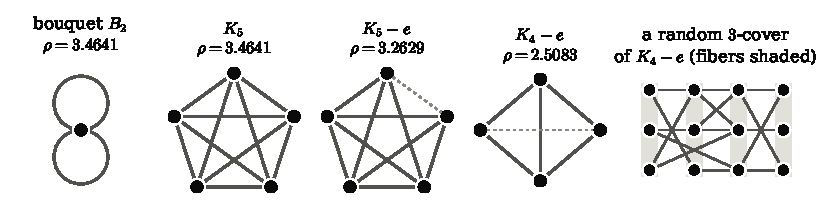
\includegraphics[width=0.98\columnwidth]{images/base_graphs_and_a_cover.pdf}
\par\end{centering}
\caption{\label{fig:bases}The base graphs of the dataset, with the spectral
radius $\rho$ of each universal cover: the bouquet of two loops,
whose random covers are the permutation model of random $4$-regular
graphs, the complete graph $K_{5}$, and the irregular graphs $K_{5}-e$
and $K_{4}-e$ (the removed edge dotted). Right: a random $3$-cover
of $K_{4}-e$, drawn with the fiber over each base vertex as a column.}
\end{figure}

The spectrum of a $\Gamma$-cover organizes along the irreducible
representations of $\Gamma$. Decomposing the permutation action
of $\Gamma$ on its group algebra into irreducibles, the adjacency
matrix of $H$ is conjugate to a direct sum
\begin{equation}
A_{H}\cong\bigoplus_{\rho\in\mathrm{Irr}(\Gamma)}A_{\rho}^{\oplus d_{\rho}},\ \ \ A_{\rho}=\sum_{e=(u,v)}E_{uv}\otimes\rho(\sigma_{e}),\label{eq:isotypic_decomposition}
\end{equation}
where the sum runs over the oriented edges of $B$, $E_{uv}$ is the
matrix unit, and $d_{\rho}$ is the dimension of $\rho$, so that
$A_{\rho}$ is an $nd_{\rho}$ dimensional Hermitian matrix (see \cite[Section 2]{HallPuderSawin2018}
for this decomposition, \cite{AgarwalChandrasekaranKollaMadan2019}
for its use on group based lifts, and \cite{BandParzanchevskiBenShach2009,Terras2010}
for its counterparts for quantum graphs and graph zeta functions).
The trivial representation recovers the base, $A_{1}=A_{B}$, and
so the new spectrum of $H$ is the union of the spectra of the non-trivial
blocks $A_{\rho}$, each with multiplicity $d_{\rho}$. Note that
the blocks of complex conjugate representations satisfy $A_{\bar{\rho}}=\overline{A_{\rho}}$
and have identical spectra, and so the distinct sources of randomness
are indexed by the non-trivial representations up to conjugation.
For a full symmetric cover the same decomposition applies with $\Gamma=S_{k}$
acting on $\{1,\dots,k\}$: the permutation representation splits
as the trivial plus the standard $(k-1)$ dimensional representation,
and the new spectrum is the single block of the standard representation.

The Frobenius-Schur indicator
\[
\varepsilon(\rho)=\frac{1}{|\Gamma|}\sum_{g\in\Gamma}\chi_{\rho}(g^{2})\in\{1,0,-1\}
\]
sorts the irreducible representations into real ($\varepsilon=1$),
complex ($\varepsilon=0$), and quaternionic ($\varepsilon=-1$) types,
and correspondingly sorts the blocks $A_{\rho}$ into the three classical
matrix symmetry classes: a real representation may be realized over
$\mathbb{R}$, making $A_{\rho}$ conjugate to a real symmetric matrix,
a complex representation gives a complex Hermitian block with no further
symmetry, and a quaternionic representation gives a self-dual block,
an $nd_{\rho}/2$ dimensional Hermitian matrix over $\mathbb{H}$,
whose eigenvalues carry an even multiplicity. In random matrix theory
these are the symmetry classes of the GOE, GUE, and GSE, whose largest
eigenvalues fluctuate according to the Tracy-Widom laws \cite{TracyWidom1994,TracyWidom1996}.
Our families realize all three types: for $\Gamma=\mathbb{Z}_{k}$
the non-trivial characters $\chi_{j}(x)=e^{2\pi ijx/k}$ give $n$
dimensional blocks with entries $\chi_{j}(\sigma_{e})$ on the edges
of the base, complex Hermitian in general and real symmetric exactly
when $\chi_{j}=\pm1$ is real valued, while the quaternion group $Q_{8}$
has a unique non-trivial higher dimensional representation, the two
dimensional representation of quaternionic type, whose real form is
four dimensional. As $k$ grows, the $\mathbb{Z}_{k}$ blocks approach
the regular graphs with independent uniform phases on the edges studied
by Oren, Godel, and Smilansky \cite{OrenGodelSmilansky2009,OrenSmilansky2010},
who compared their bulk statistics with the GUE.

Concretely, $\mathbb{Z}_{3}$ has one conjugate pair of complex characters,
and so the largest new eigenvalue of a random $\mathbb{Z}_{3}$ cover
is the largest eigenvalue of a single GUE class block. $\mathbb{Z}_{4}$
has the real character $\chi_{2}=(-1)^{x}$ together with one conjugate
pair, and so its largest new eigenvalue is the maximum of a GOE class
and a GUE class maximum. $\mathbb{Z}_{5}$ has two conjugate pairs,
giving the maximum of two GUE class maxima with identical marginal
distributions. In general, the non-trivial characters of $\mathbb{Z}_{k}$
form $\left\lfloor (k-1)/2\right\rfloor $ conjugate pairs, together
with the real character $\chi_{k/2}(x)=(-1)^{x}$ when $k$ is even,
and so the largest new eigenvalue of a random cyclic cover is the
maximum of $\left\lfloor (k-1)/2\right\rfloor $ independent GUE
class maxima and, for even $k$, one GOE class maximum, with limiting
Ramanujan probability
\[
F_{2}(0)^{\frac{k-1}{2}}\ \ \ \text{for odd }k,\ \ \ F_{1}(0)\,F_{2}(0)^{\frac{k-2}{2}}\ \ \ \text{for even }k
\]
under Conjecture \ref{conj:ramanujan_probabilities}. The quaternion
family samples the four dimensional real form of the quaternionic
block of a random $Q_{8}$-cover directly, a $4n$ dimensional matrix
all of whose eigenvalues are new, with each distinct eigenvalue repeated
by the quaternionic structure, and so $N_{\rho}=n$. These five families,
together with the permutation covers of the bouquet (random $4$-regular
graphs), of $K_{5}$, of $K_{5}$ minus an edge, and of $K_{4}$ minus
an edge, are the subject of sections \ref{sec:regular} through \ref{sec:irregular}.

\subsection{\label{subsec:laws}The Limit Laws and the Scale Constants}

By $TW_{\beta}$ we mean the Tracy-Widom law in the original normalization
of Tracy and Widom \cite{TracyWidom1994,TracyWidom1996}, with distribution
function $F_{\beta}$, mean $\mu_{TW_{\beta}}$, and standard deviation
$\sigma_{TW_{\beta}}$, and by $\widetilde{TW}_{\beta}$ the standardization
to mean $0$ and variance $1$. The constants we use are
\begin{equation}
\begin{array}{ccccc}
\beta & \mu_{TW_{\beta}} & \sigma_{TW_{\beta}} & \left|\mu_{TW_{\beta}}\right|/\sigma_{TW_{\beta}} & F_{\beta}(\mu_{TW_{\beta}})\\
1 & -1.2065335746 & 1.2679830577 & 0.9515376 & 0.519652\\
2 & -1.7710868074 & 0.9017731382 & 1.9640048 & 0.515016\\
4 & -2.3068848932 & 0.7195302084 & 3.2060987 & 0.511069
\end{array}\label{eq:tw_constants}
\end{equation}
following \cite{Bornemann2010Fredholm,Bornemann2010Review}, and the
values $F_{1}(0)=0.8319081\dots$, $F_{2}(0)=0.96937\dots$, $F_{4}(0)=0.99857\dots$
of the distribution functions at the origin. We evaluate $F_{\beta}$
as Fredholm determinants by Gauss-Legendre quadrature, following Bornemann
\cite{Bornemann2010Fredholm}, which is accurate to near machine precision
and so usable deep into both tails, and which reproduces every constant
in (\ref{eq:tw_constants}) to the digits shown. Figure \ref{fig:tw_laws}
shows the three densities, and the maximum laws of section \ref{subsec:mixed}.

\begin{figure}[tbp]
\begin{centering}
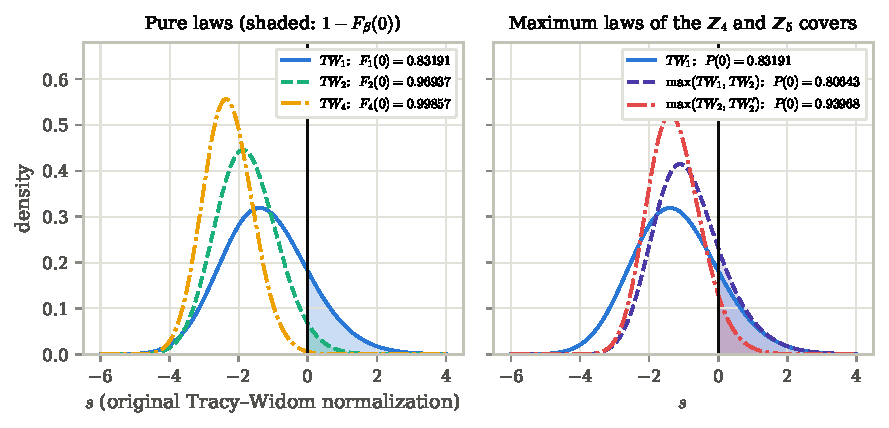
\includegraphics[width=0.95\columnwidth]{images/tracy_widom_laws_and_ramanujan_functionals.pdf}
\par\end{centering}
\caption{\label{fig:tw_laws}Left: the densities of $TW_{1}$, $TW_{2}$, and
$TW_{4}$ in the original normalization, with the mass $1-F_{\beta}(0)$
to the right of the origin shaded, the limiting probability that a
block of class $\beta$ is not Ramanujan. Right: the densities of
the maximum laws of the $\mathbb{Z}_{4}$ and $\mathbb{Z}_{5}$ covers,
against $TW_{1}$.}
\end{figure}

The scales in Conjecture \ref{conj:symmetry_classes} refer to the
Gaussian ensembles normalized alike. Let $N^{2/3}(\lambda_{\max}-2)\rightarrow\chi_{\beta}$
for the Gaussian ensemble of class $\beta$ and dimension $N$ over
$\mathbb{R}$, $\mathbb{C}$, or $\mathbb{H}$, normalized so that
its semicircle law is supported on $[-2,2]$. For $\beta=1,2$ this
is the definition of $TW_{\beta}$, while for $\beta=4$ Tracy and
Widom normalized the GSE differently \cite[Section VII]{TracyWidom1996}.
In the notation of Bornemann's review, the soft edge limit of the
GSE of complex dimension $2N$ is taken at $\sqrt{4N}$ on the scale
$2^{-1/2}(2N)^{-1/6}$ \cite[(2.4)]{Bornemann2010Review}, and $F_{4}(s)$
is its distribution function evaluated at $\sqrt{2}s$ \cite[(2.10)]{Bornemann2010Review}.
Rescaling the edge $\sqrt{4N}$ to $2$ gives
\[
\chi_{4}=2^{-2/3}\sqrt{2}\,TW_{4}=2^{-1/6}\,TW_{4}.
\]
A direct simulation of $2\times10^{4}$ samples of this ensemble with
$N=200$ gives a standard deviation of $0.6417$ for $N^{2/3}(\lambda_{\max}-2)$,
against $2^{-1/6}\sigma_{TW_{4}}=0.6410$, while the same simulation
of the GOE and GUE gives $1.2620$ and $0.9054$, against $\sigma_{TW_{1}}=1.2680$
and $\sigma_{TW_{2}}=0.9018$.

The scale constants themselves come from the square root edge of the
limiting spectral measure, as in (\ref{eq:kesten_mckay_edge}). For
a base graph $B$, the measure $\mu_{B}$ of Conjecture \ref{conj:irregular_base}
is computable from the branch values $y_{u\rightarrow v}(z)$, the
solution with positive imaginary part for $\mathrm{Im}\,z>0$ of
\begin{equation}
y_{u\rightarrow v}(z)=\left(z-\sum_{w\sim v,\ w\neq u}y_{v\rightarrow w}(z)\right)^{-1}\label{eq:branch_recursion}
\end{equation}
over the directed edges of $B$, since the Green's function of the
universal cover at a lift of $v$ is $G_{v}(z)=\left(z-\sum_{w\sim v}y_{v\rightarrow w}(z)\right)^{-1}$
and $d\mu_{B}/dx=-\frac{1}{\pi n}\sum_{v}\mathrm{Im}\,G_{v}(x+i0)$.
Solving (\ref{eq:branch_recursion}) by Newton's method, continued
from the upper half plane to within $10^{-12}$ of the real axis,
and extrapolating $\pi\,(d\mu_{B}/dx)/\sqrt{\rho(B)-x}$ to the edge
(Figure \ref{fig:universal_cover}), we obtain
\begin{equation}
\begin{array}{cccc}
B & \rho(B) & C_{B} & C_{B}^{-2/3}\\
K_{5} & 2\sqrt{3}=3.4641016 & 3^{1/4}=1.3160740 & 3^{-1/6}=0.8326832\\
K_{5}-e & 3.2628765 & 1.7250777 & 0.6952285\\
K_{4}-e & \sqrt{1+2\sqrt{7}}=2.5082868 & 10.2071395 & 0.2125188
\end{array}\label{eq:edge_constants}
\end{equation}
where the $K_{5}$ row recovers $C(4)$ and $c(4)$ of (\ref{eq:hmy_constants})
and (\ref{eq:kesten_mckay_edge}). By Conjecture \ref{conj:irregular_base},
the largest new eigenvalue of a random cover of $B$ on $V=nk$ vertices
is $\rho(B)+C_{B}^{-2/3}V^{-2/3}X$ with $X$ asymptotically $TW_{1}$.
Note that the square root law for $K_{4}-e$ sets in only within about
$10^{-3}$ of its edge, against $10^{-2}$ for $K_{5}-e$, which will
matter in section \ref{subsec:k4e}.

\begin{figure}[tbp]
\begin{centering}
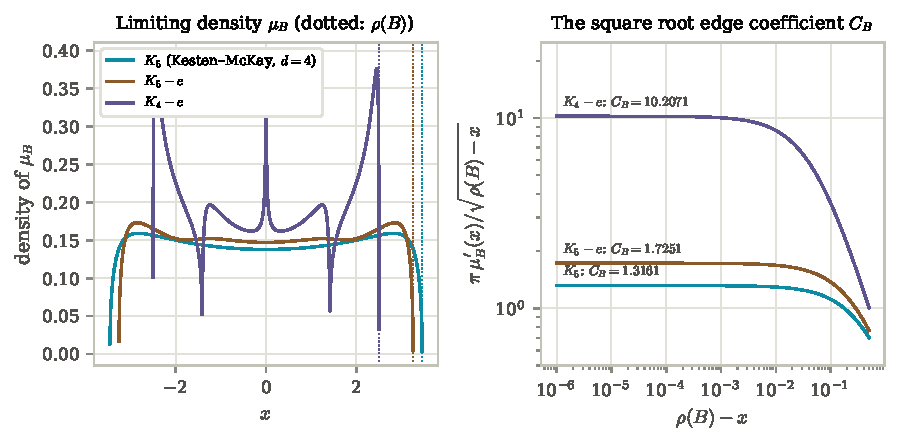
\includegraphics[width=0.95\columnwidth]{images/universal_cover_densities.pdf}
\par\end{centering}
\caption{\label{fig:universal_cover}Left: the limiting densities $\mu_{B}$
of the new eigenvalues of random covers of $K_{5}$ (the Kesten-McKay
law with $d=4$), $K_{5}-e$, and $K_{4}-e$, computed from the branch
recursion (\ref{eq:branch_recursion}), with the edges $\rho(B)$
dotted. Right: $\pi\,\mu_{B}'(x)/\sqrt{\rho(B)-x}$ against the distance
to the edge, which converges to the constant $C_{B}$ of (\ref{eq:edge_constants}).
The square root regime of $K_{4}-e$ is an order of magnitude narrower
than those of $K_{5}$ and $K_{5}-e$.}
\end{figure}


\subsection{\label{subsec:statistics}The Statistics}

For each family and size we record the sample mean $\mu_{V}$, standard
deviation $\sigma_{V}$, skewness, and excess kurtosis of the largest
new eigenvalue $\lambda$, the Kolmogorov-Smirnov distance between
the standardized sample and each of $\widetilde{TW}_{1},\widetilde{TW}_{2},\widetilde{TW}_{4}$
and the standard normal, the fraction of samples below the Ramanujan
threshold, and the fraction below the sample mean. The last statistic
is MNS's discriminator: the standardized Tracy-Widom laws are nearly
indistinguishable by their overall shape, however their masses to
the left of the mean, listed in (\ref{eq:tw_constants}), differ in
the third decimal, and with $10^{6}$ to $5\times10^{6}$ samples
the binomial standard error is between $2\times10^{-4}$ and $5\times10^{-4}$,
separating the four candidates by tens of standard errors. At MNS's
$1000$ samples per size the same separation is a third of a standard
error (Figure \ref{fig:power}).

\begin{figure}[tbp]
\begin{centering}
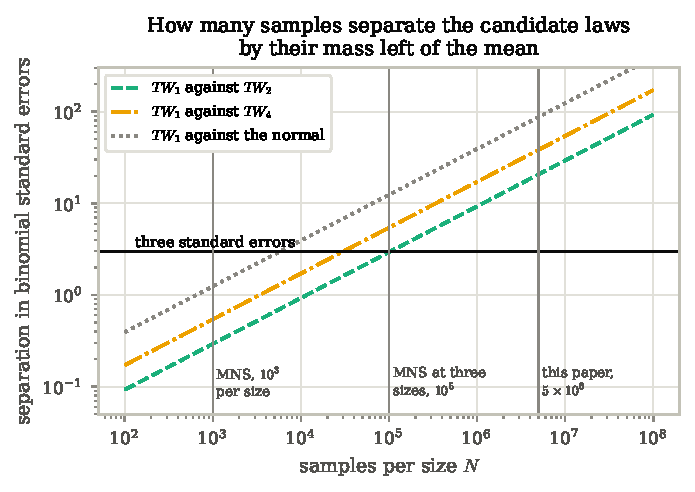
\includegraphics[width=0.7\columnwidth]{images/discriminating_power_vs_samples.pdf}
\par\end{centering}
\caption{\label{fig:power}The separation, in binomial standard errors, of
the mass of $TW_{1}$ to the left of its mean from those of $TW_{2}$,
$TW_{4}$, and the normal law, against the number $N$ of samples
per size. With $N=1000$, as in most of MNS's sizes, $TW_{1}$ and
$TW_{2}$ are separated by $0.3$ standard errors, and with our $5\times10^{6}$
by $21$.}
\end{figure}

The relevance of the ratio $g_{V}=\left(\rho-\mu_{V}\right)/\sigma_{V}$
of the mean gap to the standard deviation, with $\rho$ the family's
threshold, is the following elementary observation of MNS. For a $d$-regular
family, the probability of being one-sided Ramanujan is
\[
P\left(\lambda\leq2\sqrt{d-1}\right)=P\left(\frac{\lambda-\mu_{V}}{\sigma_{V}}\leq g_{V}\right),
\]
and so if the standardized law converges to $\widetilde{TW}_{1}$,
then
\begin{equation}
\lim_{V\rightarrow\infty}P\left(\lambda\leq2\sqrt{d-1}\right)=\begin{cases}
F_{1}(\mu_{TW_{1}})=0.519652\dots & \text{if }g_{V}\rightarrow0\\
\widetilde{F}_{1}(r) & \text{if }g_{V}\rightarrow r\in(0,\infty)\\
1 & \text{if }g_{V}\rightarrow\infty
\end{cases}.\label{eq:trichotomy}
\end{equation}
MNS's power law fits pointed to the first case. The Tracy-Widom scaling
(\ref{eq:hmy_constants}), with no shift in the centering, forces
the middle case with $r=\left|\mu_{TW_{1}}\right|/\sigma_{TW_{1}}$,
where $\widetilde{F}_{1}(r)=F_{1}(0)$, and this is what our data
shows and what Theorem \ref{thm:hmy} now proves.

Standardizing by the sample mean and standard deviation discards the
two numbers the conjectures predict, and so we also compare each sample
with its conjectured law directly. For a family whose conjectured
law is $\lambda\approx\rho+cN^{-2/3}\chi$, where $N$ is the block
dimension $N_{\rho}$ of Conjecture \ref{conj:symmetry_classes} ($N=V$
for the regular and fixed base families, and $N=n$ for the character
and quaternion blocks over a base on $n$ vertices), we form the \emph{parameter-free}
variable
\[
s=\frac{(\lambda-\rho)N^{2/3}}{c},
\]
with $c=c(4)$ for every $4$-regular family and $c=C_{B}^{-2/3}$
for the fixed bases, and nothing fitted. To separate the finite size
corrections, we regress the empirical quantiles $s_{p}$ on the quantiles
$\chi_{p}$ of the conjectured law over $0.05\leq p\leq0.95$,
\[
s_{p}\approx\alpha_{N}+\gamma_{N}\chi_{p},
\]
and report the \emph{scale ratio} $\gamma_{N}$, which should tend
to $1$, and the \emph{location coefficient} $a_{N}=-\alpha_{N}cN^{1/3}$,
defined so that the fitted law of $\lambda$ is
\begin{equation}
\lambda\approx\rho-\frac{a_{N}}{N}+\gamma_{N}\,cN^{-2/3}\chi.\label{eq:finite_size_law}
\end{equation}
Standard errors of $\gamma_{N}$ and $a_{N}$ come from ten batches
in generation order. The Kolmogorov-Smirnov distance of $(s-\alpha_{N})/\gamma_{N}$
to the conjectured law, the distance after the affine fit, then measures
the shape alone, and is unaffected by the far tails of section \ref{sec:irregular},
which move the sample moments but not the quantiles.

\subsection{\label{subsec:dataset}The Dataset and the Pipeline}

The dataset consists of $1.4\times10^{8}$ samples across ten series,
each sample the largest new eigenvalue of one independently generated
graph or cover, all with base degree $d=4$.

\begin{center}
{\footnotesize\setlength{\tabcolsep}{4pt}
\begin{tabular}{|c|c|c|c|}
\hline
family & sizes & samples & model\tabularnewline
\hline
simple $4$-regular & $100\leq V\leq20{,}000$ ($8$) & $5{,}000{,}000$ & two permutations, repaired\tabularnewline
\hline
simple $4$-regular (legacy) & $5\times10^{4}\leq V\leq5\times10^{5}$ ($4$) & $100{,}000$ & two permutations, rejection\tabularnewline
\hline
permutation multigraph & $5\times10^{4}\leq V\leq5\times10^{5}$ ($4$) & $100{,}000$ & loops and multiple edges kept\tabularnewline
\hline
$\mathbb{Z}_{k}$ covers, $k=3,4,5$ & $100\leq n\leq5000$ ($6$ each) & $1{,}000{,}000$ & random simple $4$-regular base\tabularnewline
\hline
quaternion covers & $100\leq n\leq5000$ ($6$) & $1{,}000{,}000$ & random simple $4$-regular base\tabularnewline
\hline
covers of $K_{5}$ & $100\leq V\leq10{,}000$ ($7$) & $5{,}000{,}000$ & fixed base $K_{5}$\tabularnewline
\hline
covers of $K_{5}-e$ & $100\leq V\leq10{,}000$ ($7$) & $5{,}000{,}000$ & fixed irregular base\tabularnewline
\hline
covers of $K_{4}-e$ & $100\leq V\leq10{,}000$ ($7$) & $1{,}000{,}000$ & fixed base of cycle rank two\tabularnewline
\hline
\end{tabular}}
\par\end{center}

The simple $4$-regular series draws two independent uniform permutations
$\pi_{1},\pi_{2}$ of $\{1,\dots,V\}$, forms the graph with adjacency
matrix $P_{1}+P_{1}^{T}+P_{2}+P_{2}^{T}$, and repairs it locally,
drawing each permutation in turn and repeatedly permuting its entries
at the positions that create a loop or a multiple edge, together with
one random further position, until none remains, and it discards the
rare disconnected samples. The legacy simple series instead imposes simplicity
by rejection, redrawing the whole graph. Both produce simple $4$-regular
graphs that differ from the permutation model (MNS's family $G_{V,4}$,
analyzed first by Friedman \cite{Friedman1991}, and a random degree
$V$ cover of the bouquet of two loops) in a bounded number of positions,
and the permutation model conditioned on simplicity is contiguous
with the uniform simple $4$-regular model \cite{GreenhillJansonKimWormald2002,Wormald1999},
to which Theorem \ref{thm:hmy} applies. Contiguity alone does not
transfer a limit law, and it is the data of section \ref{sec:regular}
that shows both series following the law of Theorem \ref{thm:hmy}
with its constant. The permutation multigraph series keeps the loops
and multiple edges, with a loop contributing $2$ to the diagonal.
The abelian series draw a fresh random simple $4$-regular base graph
on $n$ vertices for each batch, assign each base edge an independent
uniform voltage in $\mathbb{Z}_{k}$, and record the largest new eigenvalue
of the explicit $kn$-vertex cover, ten covers per base graph. A one
way analysis of variance across the ten covers sharing a base gives
intraclass correlations below $3\times10^{-4}$ in absolute value
at the largest size, and below $2.4\times10^{-3}$ at every size,
and so the residual randomness of the base is invisible at the fluctuation
scale and the samples may be treated as independent. The quaternion
series assigns each edge of a random simple $4$-regular base an independent
uniform element of $Q_{8}$ and records the top eigenvalue of the
resulting $4n$ dimensional real block. The fixed base series assign
each edge of $K_{5}$, of $K_{5}$ minus an edge, and of $K_{4}$
minus an edge an independent uniform permutation in $S_{k}$, and
record the largest new eigenvalue of the cover. These families are
analyzed in section \ref{sec:irregular}.

We compute eigenvalues with the implicitly restarted Lanczos method
(ARPACK), applied to the adjacency matrix shifted by a small multiple
of the identity so that the algebraically largest eigenvalues dominate
in magnitude. We remove old eigenvalues by comparing against the
base spectrum, computed exactly, with a tolerance of $10^{-10}$.
The number of computed eigenvalues per graph starts at $2$ and grows
automatically whenever every computed eigenvalue is old. For the regular
families this removes the trivial eigenvalue $d$ and yields $\lambda_{2}$.
For a disconnected cover, whose spectrum contains that of $B$ twice,
removal by value discards the second copy as well, an event of probability
$O(k^{1-r(B)})$ by Proposition \ref{prop:defect_counting} below,
where $r(B)$ is the cycle rank of $B$. Two precision caveats apply.
The legacy series were generated years earlier in MATLAB and are recorded
on a $10^{-12}$ grid, coarser than machine precision. A per process
seeding scheme caused seed collisions between worker tasks in the
abelian series: of its $1.8\times10^{6}$ base graph batches, $452{,}508$
($25\%$) are redundant copies of another batch, concentrated at the
smallest sizes ($55$ to $81\%$ of batches at $n\in\{100,200\}$,
and below $0.1\%$ at $n\geq1000$), so that the effective number
of independent samples at the smallest sizes is smaller than the nominal
$10^{6}$. Duplicated batches agree to better than $3\times10^{-13}$,
and dropping them moves every statistic quoted in this paper by at
most two units in its final displayed digit, consistent with the sampling
fluctuation of the removed samples. We verified every summary statistic
by independent recomputation from the raw samples. The complete dataset,
the generation code, and the analysis pipeline that produces every
figure and table of this paper are available at \url{https://github.com/enaslund/random-graphs}.

\section{\label{sec:regular}The Regular Graph Control Experiment}

In this section we test the pipeline against Theorem \ref{thm:hmy}
along the two simple $4$-regular series, measure the finite size
law, diagnose the artifact behind MNS's $52\%$, and show that the
permutation multigraph, whose moments misbehave, has the same law
in its bulk.

\subsection{Convergence to the Proven Law}

For $d=4$ we have that $c(4)=3^{-1/6}=0.8326831\dots$, and so the
proven amplitudes of the mean gap and standard deviation are
\begin{equation}
2\sqrt{3}-\mu_{V}\approx1.0046602\,V^{-2/3},\ \ \ \sigma_{V}\approx1.0558282\,V^{-2/3}.\label{eq:d4_amplitudes}
\end{equation}
The most direct test uses no fitted parameter at all. Figure \ref{fig:paramfree_simple}
compares the distribution function of $s=(\lambda_{2}-2\sqrt{3})V^{2/3}/c(4)$
with $F_{1}$ at five sizes: the scale is right, with the scale ratio
$\gamma_{V}$ descending from $1.117$ at $V=100$ to $1.0031\pm0.0003$
at $V=20{,}000$ and equal to $1.0036\pm0.0033$ at $V=500{,}000$,
and a fit $c+bV^{-2/3}$ to the fitted amplitudes $\gamma_{V}c(4)$
extrapolates to $0.8318$ to $0.8321$, against $c(4)=0.8326832$.
What remains is a shift, which we analyze in subsection \ref{subsec:finite_size},
and after it the differences left by the scale and shape corrections
are below $0.006$ from $V=5000$ on.

\begin{figure}[tbp]
\begin{centering}
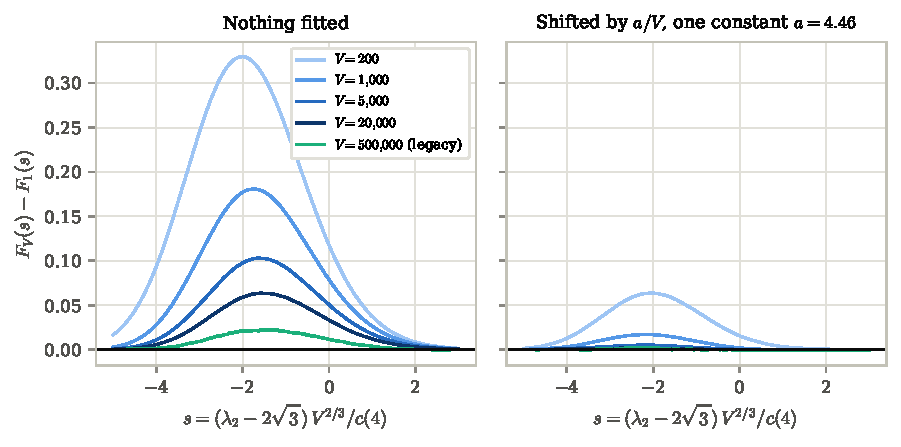
\includegraphics[width=0.95\columnwidth]{images/paramfree_simple_regular.pdf}
\par\end{centering}
\caption{\label{fig:paramfree_simple}The random simple $4$-regular graphs
against Theorem \ref{thm:hmy} with nothing fitted: $F_{V}(s)-F_{1}(s)$,
where $F_{V}$ is the empirical distribution function of $s=(\lambda_{2}-2\sqrt{3})V^{2/3}/c(4)$.
Left: the raw differences, a shift which shrinks with $V$. Right:
the same after shifting every size by $a/V$, with the single constant
$a$ of subsection \ref{subsec:finite_size}.}
\end{figure}

The standardized statistics tell the same story. Figure \ref{fig:pdf_simple}
shows the standardized empirical density of $5\times10^{6}$ samples
at $V=20{,}000$ against the four standardized candidate laws, and
Figure \ref{fig:qq_matlab} the quantile-quantile plot of the largest
legacy dataset, $V=500{,}000$, against $\widetilde{TW}_{1}$ across
the probability range $10^{-4}$ to $0.999$. The Kolmogorov-Smirnov
distances in Figure \ref{fig:ks_simple} quantify the picture across
all sizes: the distance to $\widetilde{TW}_{1}$ falls with $V$ to
the sampling floor, reaching $8.7\times10^{-4}$ at $V=20{,}000$
(the floor at $5\times10^{6}$ samples is roughly $4\times10^{-4}$),
while the distances to $\widetilde{TW}_{2}$, $\widetilde{TW}_{4}$,
and the normal stall at $3.9\times10^{-3}$, $7.8\times10^{-3}$,
and $1.9\times10^{-2}$ respectively. At the legacy sizes the sample
is statistically indistinguishable from the law: at $V=500{,}000$
the Kolmogorov-Smirnov test accepts $\widetilde{TW}_{1}$ with $p=0.99$.
The mass to the left of the mean, MNS's decisive statistic, reaches
$0.51885$ at $V=20{,}000$ and $0.52011$ at $V=500{,}000$ against
the $TW_{1}$ value $0.519652$ from (\ref{eq:tw_constants}), with
the competing values $0.515016$, $0.511069$, and $0.5$ excluded
by more than fifteen binomial standard errors (see Figure \ref{fig:mass_left}
in section \ref{sec:covers}). The sample skewness and excess kurtosis
at the largest sizes, $0.286$ and $0.156$ at $V=20{,}000$, converge
to the $TW_{1}$ values $0.293$ and $0.165$ (Figure \ref{fig:moments},
also in section \ref{sec:covers}).

\begin{figure}[tbp]
\begin{centering}
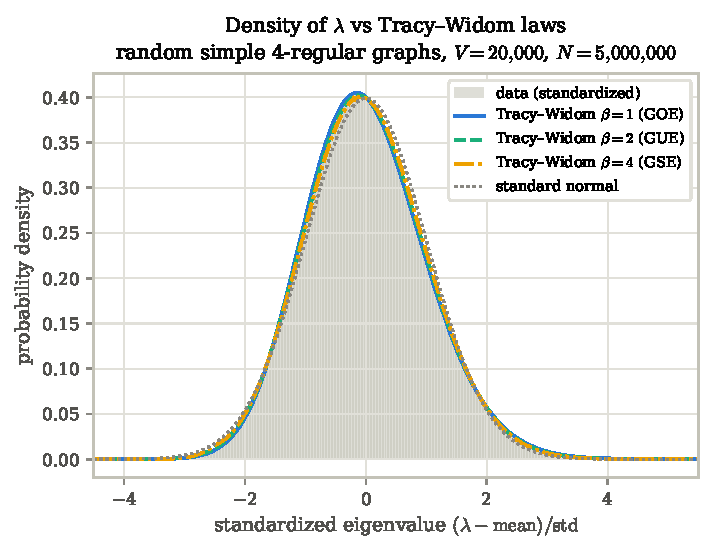
\includegraphics[width=0.75\columnwidth]{images/pdf_vs_tracywidom_simple_V20000_N5000000.pdf}
\par\end{centering}
\caption{\label{fig:pdf_simple}Standardized empirical density of the largest
non-trivial eigenvalue over $5\times10^{6}$ random simple $4$-regular
graphs on $V=20{,}000$ vertices, against the standardized Tracy-Widom
$\beta=1,2,4$ densities and the standard normal.}
\end{figure}

\begin{figure}[tbp]
\begin{centering}
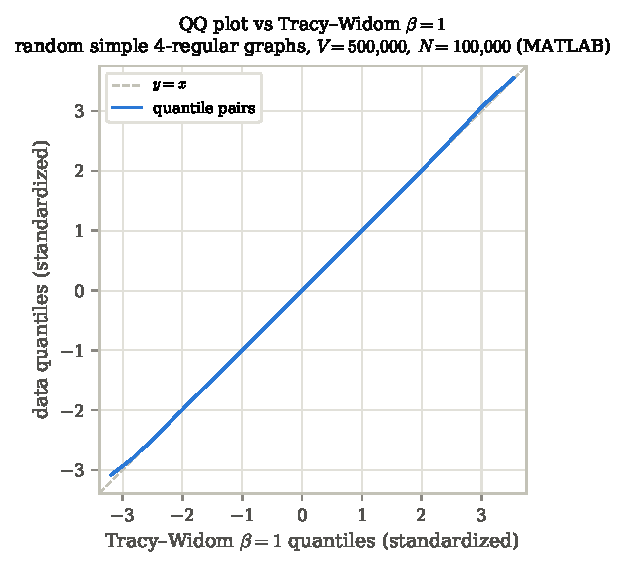
\includegraphics[width=0.6\columnwidth]{images/qq_vs_tracywidom1_matlab_simple_V500000_N100000.pdf}
\par\end{centering}
\caption{\label{fig:qq_matlab}Quantile-quantile plot of $10^{5}$ samples
at $V=500{,}000$ against $\widetilde{TW}_{1}$, probability range
$10^{-4}$ to $0.999$.}
\end{figure}

\begin{figure}[tbp]
\begin{centering}
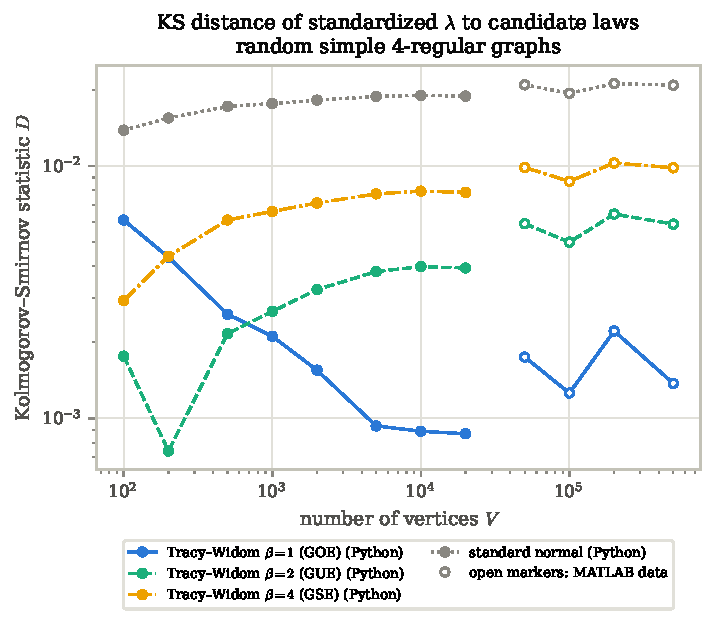
\includegraphics[width=0.75\columnwidth]{images/ks_statistic_vs_size_simple_regular.pdf}
\par\end{centering}
\caption{\label{fig:ks_simple}Kolmogorov-Smirnov distance of the standardized
samples to the standardized Tracy-Widom $\beta=1,2,4$ laws and the
standard normal, for random simple $4$-regular graphs (filled markers:
$5\times10^{6}$ samples per size, open markers: legacy data with
$10^{5}$ samples). Only the distance to $\beta=1$ keeps falling.}
\end{figure}

Figure \ref{fig:scaling_regular} shows the mean gap and standard
deviation against $V$ on logarithmic axes with the $V^{-2/3}$ guide,
and Figure \ref{fig:compensated} shows the compensated quantities
$\left(2\sqrt{3}-\mu_{V}\right)V^{2/3}$ and $\sigma_{V}V^{2/3}$,
which approach the two constants of (\ref{eq:d4_amplitudes}): at
$V=500{,}000$ the measured standard deviation is $1.685\times10^{-4}$
against the predicted $1.676\times10^{-4}$, and the measured gap
is $1.684\times10^{-4}$ against the predicted $1.595\times10^{-4}$,
the mean converging visibly more slowly than the standard deviation,
by exactly the shift $a/V$ of subsection \ref{subsec:finite_size}.
The constants (\ref{eq:d4_amplitudes}) appear in Sodin's work \cite{Sodin2009TracyWidom}
on a closely related model in which the matrix entries carry independent
random signs. We note that the arXiv posting of \cite{Sodin2009TracyWidom}
was withdrawn over an error in one of its lemmas, and the published
version carries a 2017 erratum, so that Theorem \ref{thm:hmy} is
the rigorous source for (\ref{eq:hmy_constants}).

\begin{figure}[tbp]
\begin{centering}
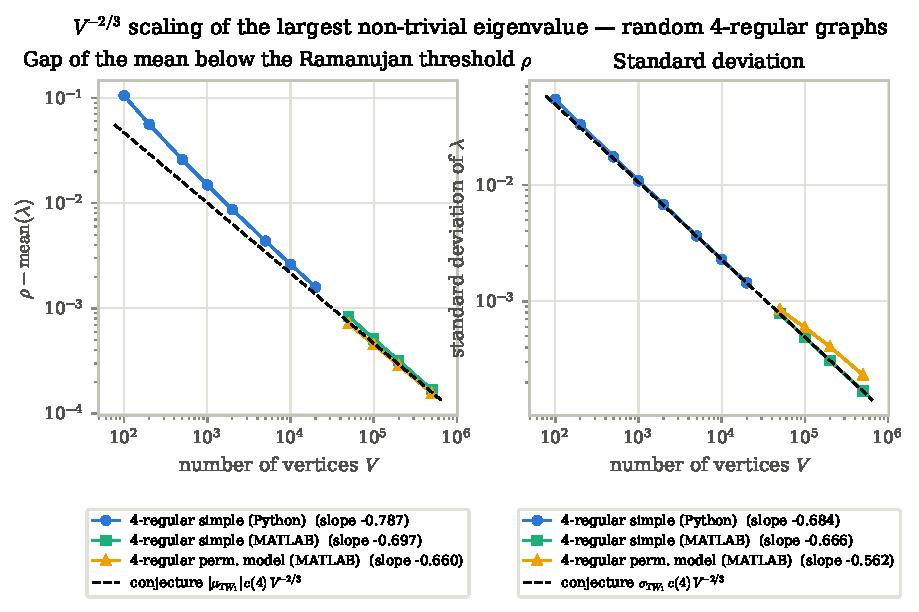
\includegraphics[width=0.8\columnwidth]{images/scaling_loglog_regular_graphs.pdf}
\par\end{centering}
\caption{\label{fig:scaling_regular}Mean gap $2\sqrt{3}-\mu_{V}$ and standard
deviation against $V$ for the three $4$-regular series, with fitted
slopes and the $V^{-2/3}$ Tracy-Widom line.}
\end{figure}

\begin{figure}[tbp]
\begin{centering}
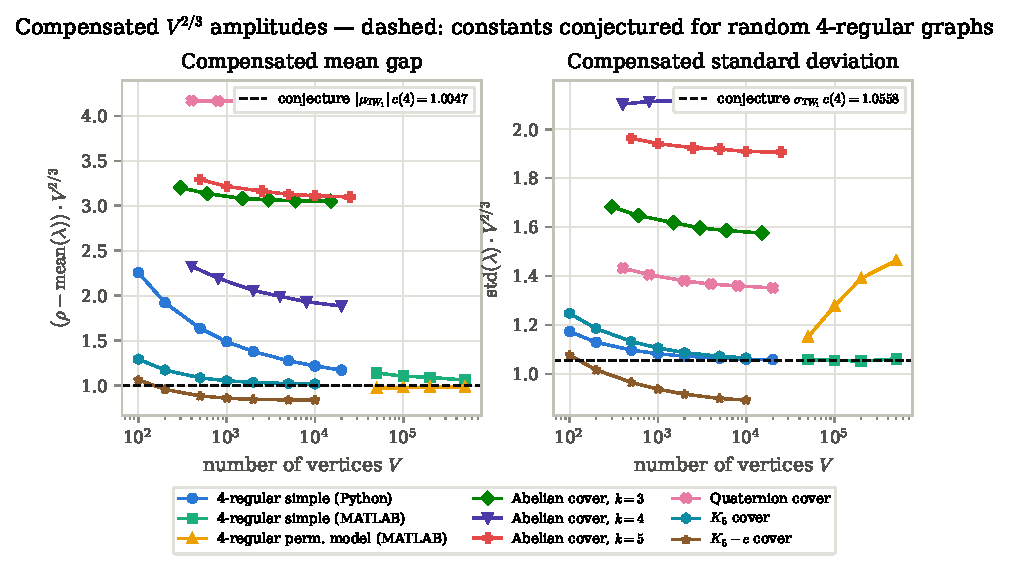
\includegraphics[width=0.8\columnwidth]{images/compensated_scaling_all_families.pdf}
\par\end{centering}
\caption{\label{fig:compensated}Compensated scaling: $\left(\rho-\mu_{V}\right)V^{2/3}$
and $\sigma_{V}V^{2/3}$ against $V$ for all families, where $\rho$
is the family's Ramanujan threshold. The dashed lines are the regular
graph amplitudes (\ref{eq:d4_amplitudes}), which the simple $4$-regular
and $K_{5}$ cover series approach, while each remaining family plateaus
at its own amplitude, predicted by Conjectures \ref{conj:symmetry_classes}
and \ref{conj:irregular_base} (see sections \ref{sec:covers} and
\ref{sec:irregular}).}
\end{figure}


\subsection{\label{subsec:finite_size}The Finite Size Law}

The theorems give no rate of convergence, and the data is precise
enough to measure the finite size law itself. Figure \ref{fig:paramfree_simple}
shows that its leading term is a shift: with $a_{V}$ the location
coefficient of (\ref{eq:finite_size_law}), the simple $4$-regular
series gives $a_{V}=5.24$ at $V=100$, $4.54$ at $V=1000$, and then
$4.479$, $4.461$, and $4.453$ at $V=5000$, $10{,}000$, and $20{,}000$,
with standard errors between $0.01$ and $0.02$, and so, with $a$ the
weighted mean over $V\geq5000$,
\begin{equation}
\lambda_{2}\approx2\sqrt{3}-\frac{a}{V}+c(4)V^{-2/3}TW_{1},\ \ \ a=4.465\pm0.008.\label{eq:shift_law}
\end{equation}
In units of the fluctuation scale this is a shift of $a/(c(4)V^{1/3})$,
which is $0.20$ at $V=20{,}000$ and $0.07$ at $V=500{,}000$, and
the scale correction is much smaller, with $\gamma_{V}-1$ decaying
roughly like $V^{-2/3}$. The shift is not a property of the degree
alone. The permutation multigraph, the same model without the conditioning,
has $a=-1.44\pm0.10$ (subsection \ref{subsec:multigraph}), the covers
of the $4$-regular graph $K_{5}$ have $a$ between $0.01$ and $0.07$
from $V=1000$ on, and the legacy simple series, which imposes simplicity
by rejection rather than by local repair, gives $a=4.87\pm0.12$
over its four sizes,
a difference of $3.4$ standard errors from (\ref{eq:shift_law})
that we do not regard as established. Conditioning on simplicity thus
moves the whole law down by about $6/V$. A shift of order $1/V$
is what one expects from the short cycles: in the physics literature,
Metz, Parisi, and Leuzzi \cite{MetzParisiLeuzzi2014} computed the
$1/V$ correction to the Kesten-McKay density of random regular graphs
as a sum over cycle lengths, with an inverse square root singularity
at the edge, which is the form of a deterministic shift of the edge
at order $1/V$, and conditioning on simplicity removes the cycles
of length one and two. For sparse Erd\H{o}s-R\'{e}nyi graphs the
corresponding deterministic shift of the edge is proven \cite{LeeSchnelli2018,BuchtSchnelliXu2025}.

\begin{figure}[tbp]
\begin{centering}
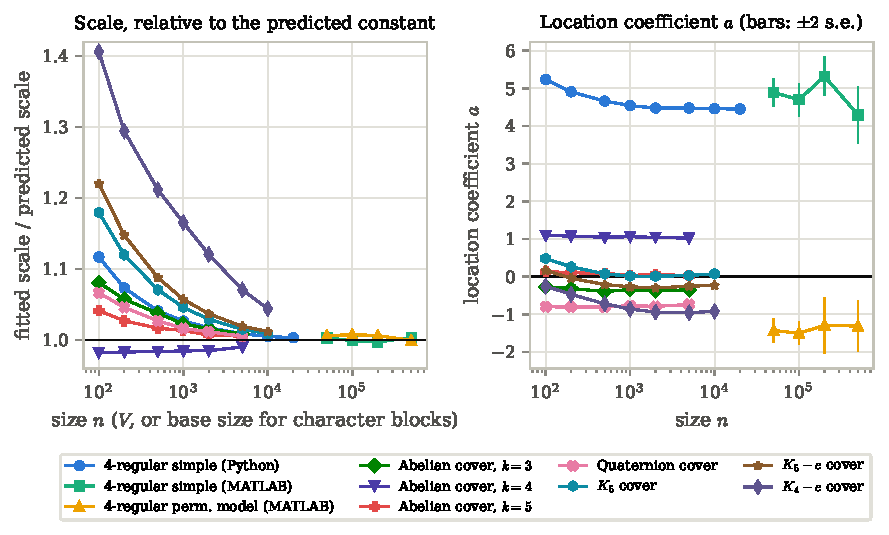
\includegraphics[width=0.95\columnwidth]{images/finite_size_scale_and_location.pdf}
\par\end{centering}
\caption{\label{fig:scale_location}The two finite size parameters of (\ref{eq:finite_size_law})
for every family, from the quantile regression of the parameter-free
variable on the conjectured law. Left: the scale ratio, the fitted
scale over the predicted one, which is $c(4)$ for the $4$-regular
families, $c(4)2^{-1/6}$ in terms of $TW_{4}$ for the quaternion
covers, and $C_{B}^{-2/3}$ of (\ref{eq:edge_constants}) for $K_{5}-e$
and $K_{4}-e$. Right: the location coefficient $a$, in the law $\rho-a/N+\gamma cN^{-2/3}\chi$,
which settles at a family dependent constant.}
\end{figure}

The shift controls the Ramanujan probability, which by (\ref{eq:shift_law})
is
\begin{equation}
P\left(\lambda_{2}\leq2\sqrt{3}\right)\approx F_{1}\left(\frac{a}{c(4)V^{1/3}}\right)=F_{1}(0)+\frac{0.9728}{V^{1/3}}+O\left(V^{-2/3}\right),\label{eq:ramanujan_rate}
\end{equation}
where $0.9728=f_{1}(0)a/c(4)$ and $f_{1}(0)=0.18142$ is the density
of $TW_{1}$ at the origin. With the single constant (\ref{eq:shift_law}),
the left side of (\ref{eq:ramanujan_rate}) matches the data to within
$3\times10^{-4}$, or $2.4$ binomial standard errors, at every size
from $V=1000$ to $20{,}000$, and to within $2.6$ standard errors
at the four legacy sizes. The convergence to $F_{1}(0)$ is thus
slow: the Ramanujan probability of the simple model is still $0.01$
above its limit at $V=8.6\times10^{5}$, and reaches within $10^{-3}$
only at $V=9\times10^{8}$ (Figure \ref{fig:ramanujan_rate}). For
the multigraph the approach is from below, since $a<0$, and it is
within $10^{-3}$ at $V=3\times10^{7}$, while the covers of $K_{5}$,
with $a$ nearly zero, are within $10^{-3}$ from $V=1000$ on. Any
experiment on the Ramanujan probability at accessible sizes measures
$F_{\beta}$ at a shifted point, and the shift must be accounted for.

\begin{figure}[tbp]
\begin{centering}
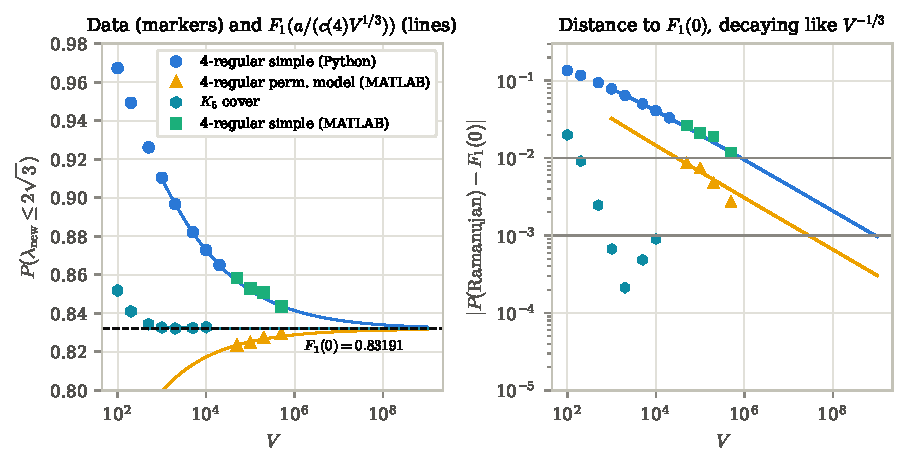
\includegraphics[width=0.95\columnwidth]{images/ramanujan_probability_rate.pdf}
\par\end{centering}
\caption{\label{fig:ramanujan_rate}Left: the empirical Ramanujan probability
against $V$ for the simple, legacy simple, multigraph, and $K_{5}$
cover series (markers), with the one parameter model $F_{1}(a/(c(4)V^{1/3}))$
of (\ref{eq:ramanujan_rate}) (lines, drawn from $V=1000$). Right:
the distance to $F_{1}(0)$ on logarithmic axes, extrapolated to $V=10^{9}$,
with the levels $10^{-2}$ and $10^{-3}$.}
\end{figure}

The third correction is to the shape. Rates at the Tracy-Widom edge
have a history in random matrix theory: Choup \cite{Choup2009} computed
the Edgeworth expansion of the largest eigenvalue law of the finite
GOE, Johnstone and Ma \cite{JohnstoneMa2012} proved that the rate
of approach depends on the centering convention, Bornemann \cite{Bornemann2026}
expanded the laws of the finite Gaussian ensembles at the soft edge
in terms of the derivatives of $F_{\beta}$, and rates of order $N^{-1/3}$ are
proven for Wigner matrices \cite{SchnelliXu2022} and sparse Erd\H{o}s-R\'{e}nyi
graphs \cite{BuchtSchnelliXu2025}. Write $F_{V}$ for the distribution
function of the standardized largest non-trivial eigenvalue and $\widetilde{F}_{1},\widetilde{f}_{1}$
for the standardized Tracy-Widom distribution and density. Standardization
removes the location and scale, and across the simple $4$-regular
family the remaining deviation $F_{V}-\widetilde{F}_{1}$ is, to within
$6$ to $14$ percent of its squared norm, proportional to the single
fixed profile $\left(t^{2}-1\right)\widetilde{f}_{1}(t)$, a correction
of Edgeworth type signaling a skewness deficit, and so to the resolution
of $5\times10^{6}$ samples the finite size law is the one parameter
family
\[
F_{V}(t)\approx\widetilde{F}_{1}(t)-\hat{c}(V)\left(t^{2}-1\right)\widetilde{f}_{1}(t),
\]
where the fitted amplitude $\hat{c}(V)$ decays like a power law with
exponent $-0.46\pm0.04$, and the $K_{5}$ cover family of section
\ref{sec:irregular} lies on the same curve (Figure \ref{fig:edgeworth}).
The same parameter accounts for the residuals of the individual standardized
statistics: the mass left of the mean at $V=20{,}000$ still sits
$-8.0\times10^{-4}$ from the $TW_{1}$ value, $3.6$ binomial standard
errors, against an Edgeworth prediction of $-\hat{c}\,\widetilde{f}_{1}(0)=-5.3\times10^{-4}$,
and after subtracting the fitted profile the left tails of the largest
datasets agree with $\widetilde{TW}_{1}$ to within three standard
errors down to probability $6\times10^{-7}$.

\begin{figure}[tbp]
\begin{centering}
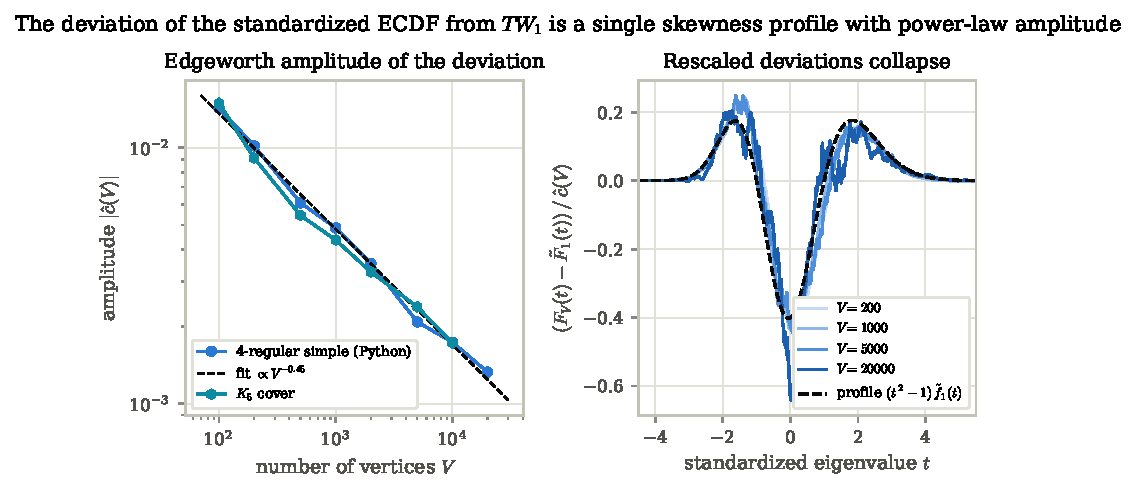
\includegraphics[width=0.85\columnwidth]{images/edgeworth_amplitude_vs_size.pdf}
\par\end{centering}
\caption{\label{fig:edgeworth}The shape correction. Left: the amplitude $\hat{c}(V)$
of the deviation of the standardized empirical distribution from $\widetilde{TW}_{1}$,
for the simple $4$-regular and $K_{5}$ cover families, with the
fitted power law. Right: the deviations at four sizes, rescaled by
$\hat{c}(V)$, collapse onto the fixed profile $\left(t^{2}-1\right)\widetilde{f}_{1}(t)$
of a skewness deficit.}
\end{figure}

\subsection{\label{subsec:mns_diagnosis}The Origin of the $52\%$ Conjecture}

MNS reached the first case of (\ref{eq:trichotomy}) by fitting single
power laws to the mean gap and standard deviation over their full
range of sizes. Our data reproduces their fit and (\ref{eq:shift_law})
explains it. Fitting one line to $\log\left(2\sqrt{3}-\mu_{V}\right)$
against $\log V$ over our eight sizes $V\leq20{,}000$, the MNS range,
gives a slope of $-0.787$, while the same fit to $\log\sigma_{V}$
gives $-0.684$: a mean exponent apparently steeper than the standard
deviation exponent, exactly the pattern from which MNS concluded $g_{V}\rightarrow0$
and hence $52\%$, with numbers closely matching their $d=3$ values
$m\approx-0.79$ and $s\approx-0.72$. Under (\ref{eq:shift_law})
the mean gap is $AV^{-2/3}+a/V$ with $A=1.0046602$ from (\ref{eq:d4_amplitudes}),
whose local exponent is
\[
\frac{d\log\left(2\sqrt{3}-\mu_{V}\right)}{d\log V}=-\frac{2/3+x}{1+x},\ \ \ x=\frac{a}{AV^{1/3}},
\]
which is $-0.72$ at $V=14{,}000$ and approaches $-2/3$ from below
only as $V^{-1/3}$. Figure \ref{fig:mns_model} compares this with
the slopes between consecutive sizes. The standard deviation exponent
sits within $0.01$ of $-2/3$ from $V\approx2000$ onward, while the
mean gap exponent drifts monotonically from $-0.90$ at $V\approx100$
to $-0.72$ at $V=20{,}000$ within the five million sample series,
with the legacy series continuing the descent and reaching $-0.70$
over its last pair at $V=500{,}000$, still short of $-2/3$, all
along the curve of the one constant model. Fitted to the model at
our eight sizes, a single power law gives $-0.764$, most of the observed
$-0.787$, the remainder coming from the larger values of $a_{V}$
at the smallest sizes. MNS saw the warning sign, observing that their
best fit exponents increased monotonically as sizes were added, and
were appropriately cautious. At $V\leq20{,}000$ the data could do
no better: by (\ref{eq:ramanujan_rate}) the Ramanujan probability
itself is $0.865$ at $V=20{,}000$, and no single size in that range
is close to the limit. The ratio $g_{V}$ resolves the question directly:
as Figure \ref{fig:ratio} shows, $g_{V}$ does not tend to $0$ for
any family, and for the simple $4$-regular series it descends to
$0.9993$ at $V=500{,}000$, approaching the Tracy-Widom ratio $\left|\mu_{TW_{1}}\right|/\sigma_{TW_{1}}=0.951537\dots$
from above, in agreement with the middle case of (\ref{eq:trichotomy})
and with $F_{1}(0)=0.8319081\dots$ as the limiting Ramanujan probability.

\begin{figure}[tbp]
\begin{centering}
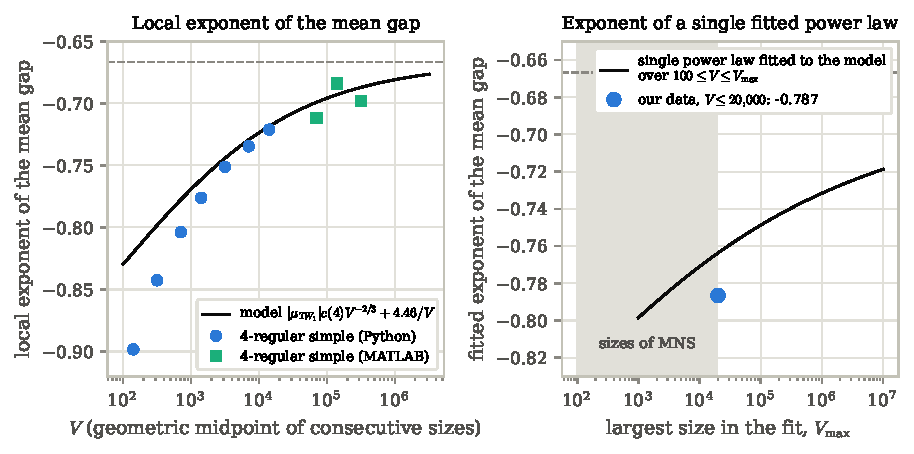
\includegraphics[width=0.95\columnwidth]{images/mns_exponent_model.pdf}
\par\end{centering}
\caption{\label{fig:mns_model}The origin of the $52\%$ conjecture. Left:
the local exponents of the mean gap between consecutive sizes for
the two simple $4$-regular series, with the prediction of the one
constant model (\ref{eq:shift_law}) and the limit $-2/3$ dashed.
Right: the exponent reported by a single power law fitted to the model
over $100\leq V\leq V_{\max}$, against $V_{\max}$, with the value
$-0.787$ fitted to our data over the sizes of MNS (shaded).}
\end{figure}

\begin{figure}[tbp]
\begin{centering}
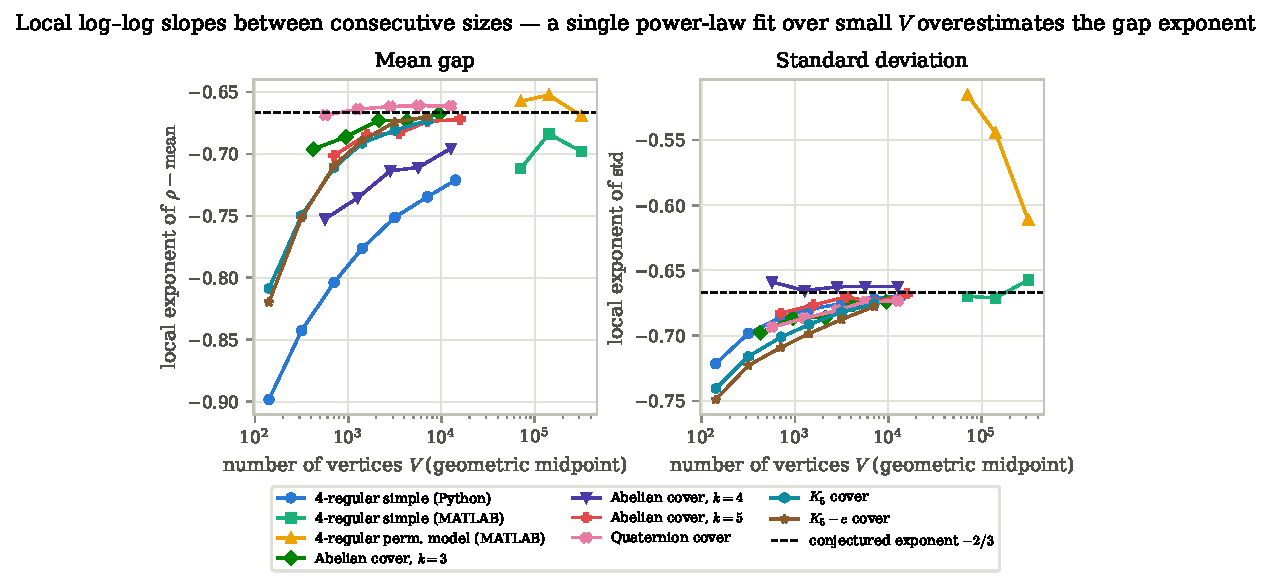
\includegraphics[width=0.8\columnwidth]{images/scaling_local_exponent_vs_size_all_families.pdf}
\par\end{centering}
\caption{\label{fig:local_exponent}Local (consecutive size) log-log exponents
of the mean gap and the standard deviation for all series, with the
$-2/3$ line. The mean gap exponent approaches $-2/3$ from below
as $V$ grows, and so a single power law fitted over small sizes overestimates
its steepness, wrongly suggesting that the gap outruns the standard
deviation.}
\end{figure}


\subsection{\label{subsec:multigraph}The Multigraph Model}

MNS pooled models with and without loops and multiple edges, observing
similar behavior at their sample sizes. At ours, the sample moments
of the permutation multigraph series, identical to the legacy simple
series except that loops and multiple edges are kept, differ qualitatively:
at $V=500{,}000$ its skewness is $74.5$ and its excess kurtosis
$1.15\times10^{4}$, against the $TW_{1}$ values $0.293$ and $0.165$,
its ratio $g_{V}$ falls through $0.67$, and the Kolmogorov-Smirnov
distance of the standardized sample to every candidate law grows with
$V$, reaching $0.085$. None of this comes from the bulk. With nothing
fitted, the parameter-free variable $s$ of the multigraph is closer
to $TW_{1}$ than that of the simple model (Figure \ref{fig:multigraph},
left), at Kolmogorov-Smirnov distance $0.0077$ against $0.0227$
at $V=500{,}000$, since its location coefficient is smaller, $a=-1.44\pm0.10$ over
the four sizes,
and its scale ratio is $0.9992\pm0.0027$. After the affine fit of
subsection \ref{subsec:statistics} the distance is $0.0016$, below
the typical value $0.0027$ for $10^{5}$ samples drawn from the law
itself. The moments are instead carried by a handful of far outliers,
a few samples in each $10^{5}$, up to about $200$ standard deviations
of the bulk above its mean at $V=500{,}000$, which inflate the sample
standard deviation by about $40\%$ and so compress the standardized
bulk.

The outliers are localized eigenvalues, and they are not produced
by the loops and multiple edges alone. A loop contributes $2$ to
the diagonal, and a loop, or a double edge, attached to the branches
of the $4$-regular tree, binds no eigenvalue above $2\sqrt{3}$,
since the resulting equation $\lambda=2+2y(\lambda)$, with $y(\lambda)=(\lambda-\sqrt{\lambda^{2}-12})/6$
the branch value of (\ref{eq:branch_recursion}), has no solution
above $2\sqrt{3}$, where its right hand side is $2+2/\sqrt{3}=3.155$.
In the language of subsection \ref{subsec:defects}, the binding defects
have cycle rank two. A triple edge, and two looped vertices joined
by an edge, each bind at exactly $7/2$, a looped vertex joined to
its neighbor by a double edge binds at the real root
\[
\lambda=3.5385847\dots\ \ \ \text{of}\ \ \ \lambda^{3}=8\lambda+16,
\]
and a triangle with a loop at one vertex binds just above the threshold,
at $3.4675039\dots$, and an exhaustive search shows that no other
defect of cycle rank two on at most five vertices binds. Of the $18$
samples more than eight standard deviations above $2\sqrt{3}$ across
the four legacy sizes, $17$ lie within $0.002$ of these three values
(Figure \ref{fig:multigraph}, right), with those on $7/2$ draining
up to it from $3.4985$ at $V=50{,}000$ to $3.4999$ at $V=500{,}000$,
and the exception, $3.5116$ at $V=50{,}000$, lies among the values
of several defects of cycle rank three. Defects of cycle rank two
occur at rate $1/V$ by Proposition \ref{prop:defect_counting}, and
so the multigraph model has least binding rank $r^{*}=2$, as does
$K_{4}-e$, and Corollary \ref{cor:moment_divergence} applies: the
defects eventually dominate the variance, growing relative to the
bulk like $V^{1/3}$, which is the growth of every moment based distance
observed above. Conditioning on simplicity removes all three defects,
and no simple subgraph of cycle rank two on at most five vertices
binds, so that the leading defect of the simple model is $K_{4}$,
which binds at $7/2$ as in the covers of $K_{5}$ but has cycle rank
three and occurs at rate $V^{-2}$. The largest sample of the simple
series at $V=500{,}000$ sits only $9$ standard deviations above
its mean.

\begin{figure}[tbp]
\begin{centering}
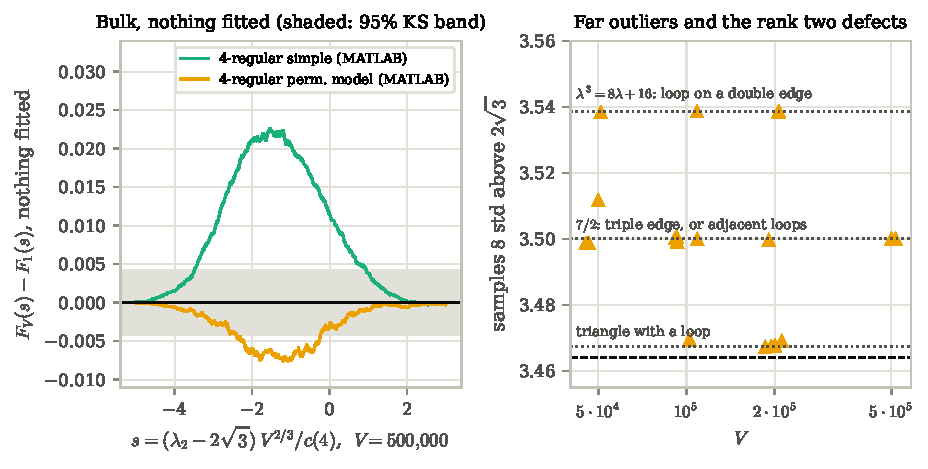
\includegraphics[width=0.95\columnwidth]{images/multigraph_model_bulk_and_atoms.pdf}
\par\end{centering}
\caption{\label{fig:multigraph}The permutation multigraph model. Left: $F_{V}(s)-F_{1}(s)$
for the parameter-free variable at $V=500{,}000$, for the multigraph
and the legacy simple series, with the $95\%$ Kolmogorov-Smirnov
band for $10^{5}$ samples shaded: nothing is fitted, and the multigraph
is closer to the law. Right: every multigraph sample more than eight
standard deviations above $2\sqrt{3}$ against $V$, with the three
computed defect eigenvalues of cycle rank two dotted.}
\end{figure}

The lesson for experiments in this area is that statistics built from
sample moments are unusable when defects of low cycle rank bind, while
quantile statistics are immune to them. The simple and multigraph
models share the limiting spectral distribution, the almost sure convergence
of $\lambda_{2}$ to $2\sqrt{3}$, and the Tracy-Widom law of the
bulk with its constant, and they are separated at the fluctuation
scale by a deterministic shift of order $1/V$ and by a thin tail
of defects of cycle rank two.

\section{\label{sec:covers}Covers and the Threefold Way}

We now turn to the main experiment. Each abelian and quaternion family
isolates a definite set of isotypic blocks, and Conjecture \ref{conj:symmetry_classes}
predicts the symmetry class of each: $\mathbb{Z}_{3}$ covers should
follow $\chi_{2}$, quaternion covers $\chi_{4}$, the regular graph
families of section \ref{sec:regular} $\chi_{1}$, and the mixed
families $\mathbb{Z}_{4}$ and $\mathbb{Z}_{5}$ no single Tracy-Widom
law at all.

\subsection{Ensemble Selection in the Pure Families}

Figure \ref{fig:ks_matrix} is the structural result of this paper.
For each family at its largest size, and for each candidate law, it
shows the Kolmogorov-Smirnov distance after the best affine fit to
that law, which removes the location and scale and compares the shapes
alone. In every row the minimum is the law of the family's own class:
$TW_{1}$ for the regular, $K_{5}$, and $K_{5}-e$ families, at $0.6$
to $0.7\times10^{-3}$, against $2.1\times10^{-3}$ or more for every
other law, $TW_{2}$ for $\mathbb{Z}_{3}$ covers, at $0.8\times10^{-3}$
against $2.6\times10^{-3}$ for $TW_{4}$ and $3.5\times10^{-3}$
for $TW_{1}$, and $TW_{4}$ for quaternion covers, at $0.5\times10^{-3}$
against $2.7\times10^{-3}$ for $TW_{2}$ and $5.6\times10^{-3}$ for
$TW_{1}$, where the typical distance of $10^{6}$ samples from their
own law is $0.9\times10^{-3}$. The mixed families select their maximum
laws in the same way (subsection \ref{subsec:mixed}).

\begin{figure}[tbp]
\begin{centering}
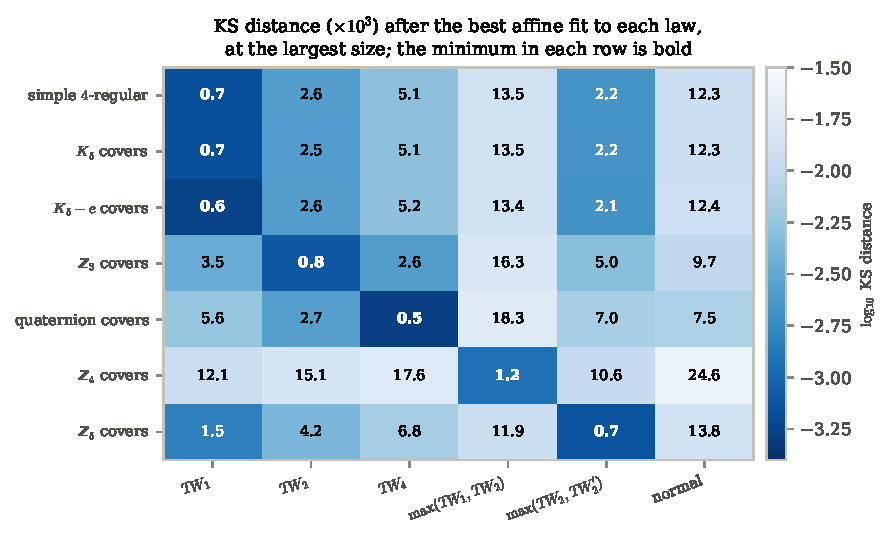
\includegraphics[width=0.8\columnwidth]{images/ks_matrix_families_vs_laws.pdf}
\par\end{centering}
\caption{\label{fig:ks_matrix}Kolmogorov-Smirnov distance, times $10^{3}$,
between each family at its largest size and each candidate law, after
the best affine fit of the sample to that law, so that only the shape
is compared. The minimum in each row, in bold, is the law predicted
by Conjectures \ref{conj:symmetry_classes}, \ref{conj:ramanujan_probabilities},
and \ref{conj:irregular_base}. The typical distance of a sample from
its own law is $0.4\times10^{-3}$ at $5\times10^{6}$ samples and
$0.9\times10^{-3}$ at $10^{6}$.}
\end{figure}

The standardized statistics agree. Figure \ref{fig:ks_classes} shows
that for each pure family the Kolmogorov-Smirnov distance to the standardized
law of its own symmetry class falls to the sampling floor while the
distance to $\widetilde{TW}_{1}$ (dotted) stalls. At the largest
sizes, the $\mathbb{Z}_{3}$ family reaches distance $1.0\times10^{-3}$
from $\widetilde{TW}_{2}$ (floor at $10^{6}$ samples: roughly $9\times10^{-4}$)
while its distance to $\widetilde{TW}_{1}$ is stuck at $5.4\times10^{-3}$,
and the quaternion family reaches $7.5\times10^{-4}$ from $\widetilde{TW}_{4}$
with distance $8.8\times10^{-3}$ to $\widetilde{TW}_{1}$. The mass
to the left of the mean (Figure \ref{fig:mass_left}) separates the
classes at higher resolution: the $\mathbb{Z}_{3}$ series converges
to $0.5145$ against the $TW_{2}$ value $0.515016$, the quaternion
series to $0.5109$ against the $TW_{4}$ value $0.511069$, and the
regular series to $0.5201$ against the $TW_{1}$ value $0.519652$,
each matching its own class, with every competing class excluded by
six or more binomial standard errors for the cover families and by
three or more for the legacy regular sample.

The tails separate the classes most visibly, since the standardized
Tracy-Widom laws differ most there, the left tail of $TW_{\beta}$
decaying like $\exp(-\beta|s|^{3}/24)$. Figure \ref{fig:tails} shows
both tails of the three pure families down to probability $10^{-6}$,
after mapping each sample onto its own law by the affine fit and standardizing:
each follows the tail of its own class. The affine invariant moments agree as
well: Figure \ref{fig:moments} shows the sample skewness and excess
kurtosis of each family converging to the values of its own class,
$\left(0.213,0.093\right)$ at the largest $\mathbb{Z}_{3}$ size
against the $TW_{2}$ values $\left(0.224,0.093\right)$, and $\left(0.156,0.042\right)$
at the largest quaternion size against the $TW_{4}$ values $\left(0.166,0.049\right)$,
and Figure \ref{fig:moment_plane} shows the same trajectories in
the plane of the two moments, where each family, the mixed ones included,
moves to the point of its own limit law. Figure \ref{fig:qq_beta}
gives the quantile level view of the same selection, and Figure \ref{fig:universality}
overlays the standardized densities of the largest datasets from five
families on the $\widetilde{TW}_{1}$ density: at the resolution of
the eye all collapse to the Tracy-Widom shape, and the discrimination
between the $\beta$ classes lives in the statistics above.

\begin{figure}[tbp]
\begin{centering}
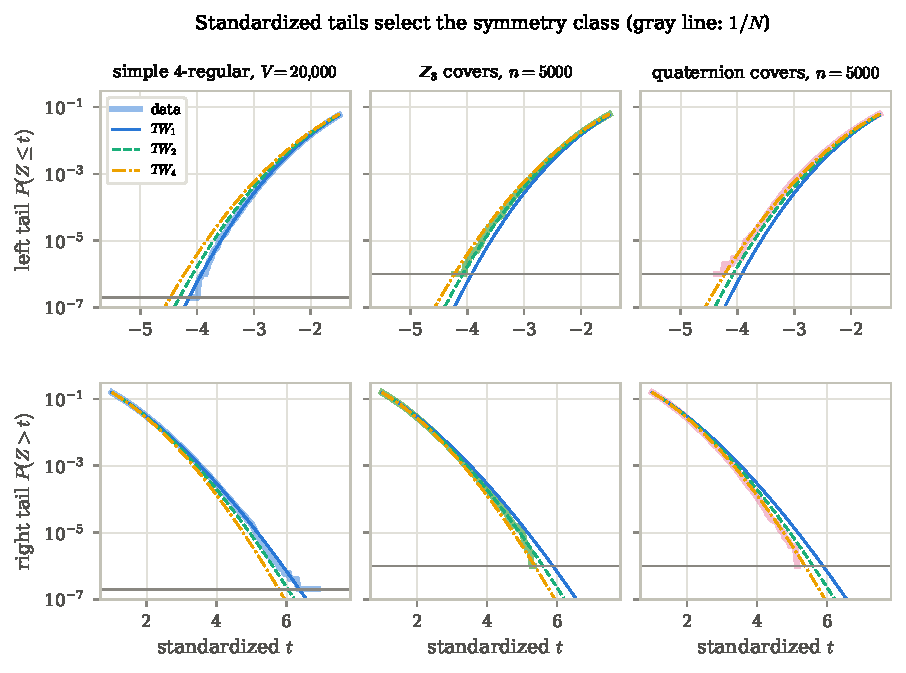
\includegraphics[width=0.95\columnwidth]{images/tails_by_symmetry_class.pdf}
\par\end{centering}
\caption{\label{fig:tails}Left tails (top) and right tails (bottom) on logarithmic
axes for the simple $4$-regular graphs at $V=20{,}000$, the $\mathbb{Z}_{3}$
covers at $n=5000$, and the quaternion covers at $n=5000$, after
the affine fit to the law of each family's class and standardization,
against the standardized $TW_{1}$, $TW_{2}$, and $TW_{4}$. The gray
line is $1/N$.}
\end{figure}

\begin{figure}[tbp]
\begin{centering}
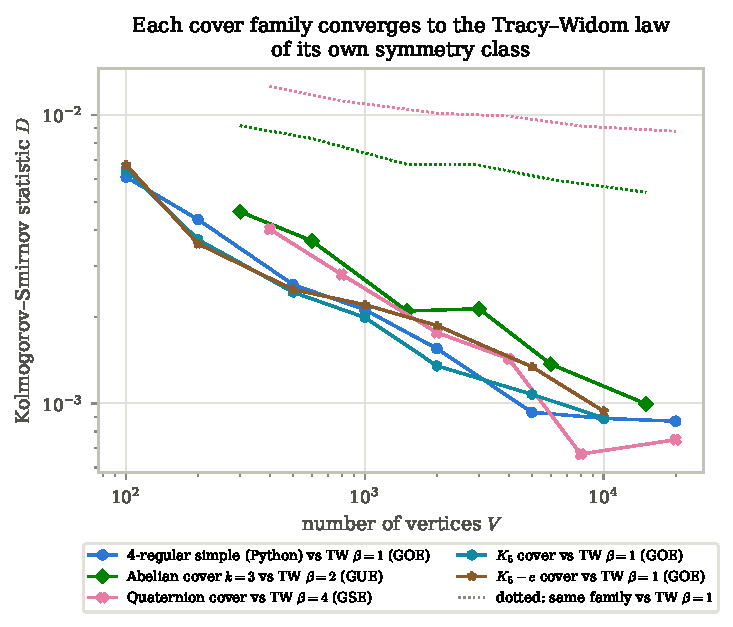
\includegraphics[width=0.8\columnwidth]{images/ks_statistic_symmetry_classes.pdf}
\par\end{centering}
\caption{\label{fig:ks_classes}Kolmogorov-Smirnov distance of each pure family
to the standardized Tracy-Widom law of its own symmetry class (solid):
regular graphs and the fixed base $K_{5}$ and $K_{5}-e$ cover families
to $\beta=1$, $\mathbb{Z}_{3}$ covers to $\beta=2$, quaternion covers
to $\beta=4$, with the distance to $\beta=1$ dotted for contrast.
The matching class distances fall to the sampling noise floor. The
mixed families $\mathbb{Z}_{4}$ and $\mathbb{Z}_{5}$ match no single
law.}
\end{figure}

\begin{figure}[tbp]
\begin{centering}
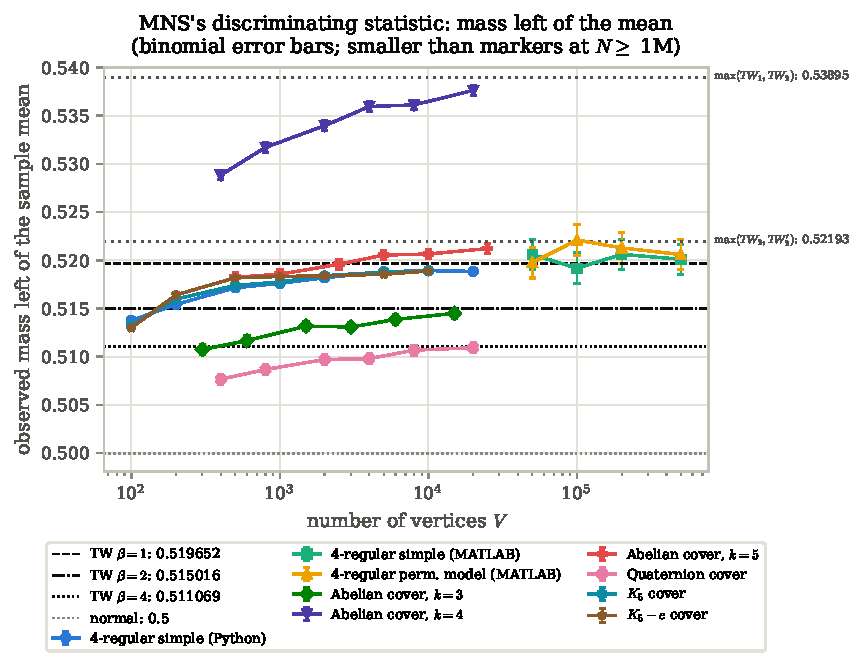
\includegraphics[width=0.8\columnwidth]{images/mass_left_of_mean_vs_size_all_families.pdf}
\par\end{centering}
\caption{\label{fig:mass_left}The fraction of samples below the sample mean
against $V$ for all families, with the Tracy-Widom $\beta=1,2,4$
and normal reference values. This replicates MNS's decisive experiment
at fifty times their sample size: with $10^{6}$ to $5\times10^{6}$
samples the binomial standard error is between $2\times10^{-4}$ and
$5\times10^{-4}$ and the four candidate laws are separated by tens
of standard errors. Each pure family selects the value of its own
symmetry class, while the mixed family $\mathbb{Z}_{4}$ drifts to
$\approx0.538$, consistent with the maximum law of Table \ref{tab:predicted_observed}
and no Tracy-Widom law.}
\end{figure}

\begin{figure}[tbp]
\begin{centering}
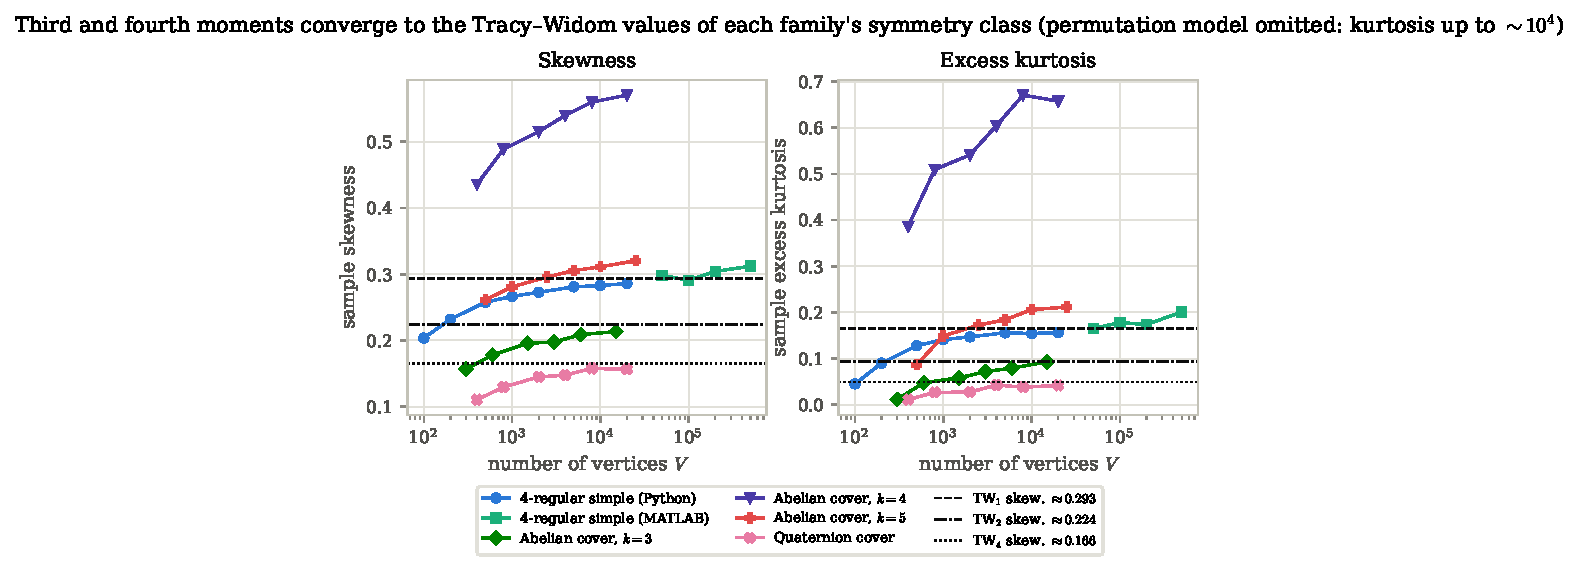
\includegraphics[width=0.8\columnwidth]{images/moments_skewness_kurtosis_vs_size.pdf}
\par\end{centering}
\caption{\label{fig:moments}Sample skewness and excess kurtosis against $V$
with the Tracy-Widom $\beta=1,2,4$ reference values. The regular
families converge to the $\beta=1$ moments, $\mathbb{Z}_{3}$ to
$\beta=2$, and quaternion to $\beta=4$. The multigraph model (excess
kurtosis up to $10^{4}$) and the fixed base cover families, whose
third and fourth moments are dominated by the far outlier tails of
section \ref{sec:irregular}, are omitted.}
\end{figure}

\begin{figure}[tbp]
\begin{centering}
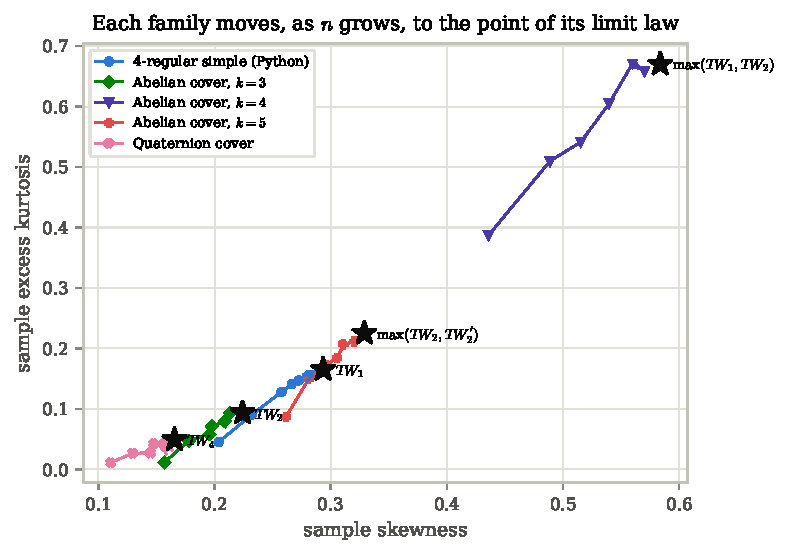
\includegraphics[width=0.7\columnwidth]{images/moment_plane_trajectories.pdf}
\par\end{centering}
\caption{\label{fig:moment_plane}Sample skewness against excess kurtosis for
the simple $4$-regular, cyclic, and quaternion families, one marker
per size, with the arrow at the largest size. Each family moves to
the point of its limit law (stars): $TW_{1}$, $TW_{2}$, $TW_{4}$,
or the maximum laws of subsection \ref{subsec:mixed}.}
\end{figure}

\begin{figure}[tbp]
\begin{centering}
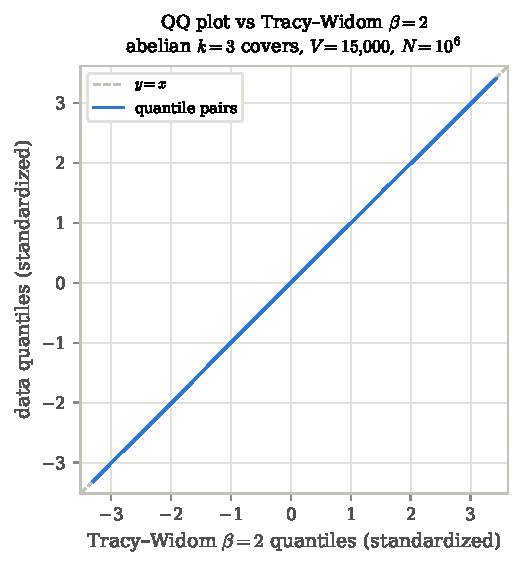
\includegraphics[width=0.42\columnwidth]{images/qq_vs_tracywidom2_abelian3_V15000_N1000000.pdf}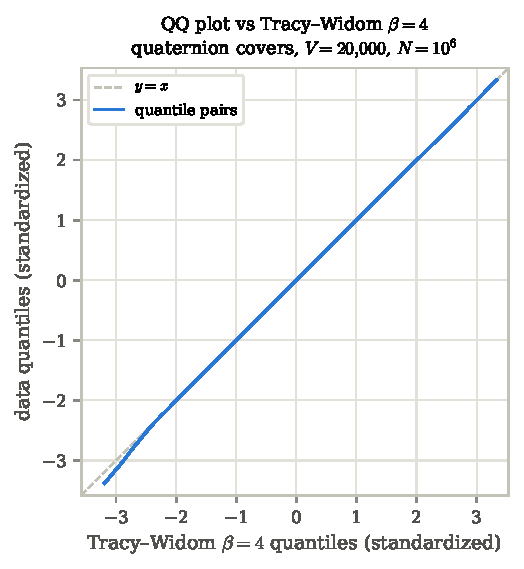
\includegraphics[width=0.42\columnwidth]{images/qq_vs_tracywidom4_quaternion_V20000_N1000000.pdf}
\par\end{centering}
\caption{\label{fig:qq_beta}Quantile-quantile plots of the largest $\mathbb{Z}_{3}$
cover dataset against Tracy-Widom $\beta=2$ (left) and of the largest
quaternion cover dataset against $\beta=4$ (right), both standardized,
probability range $10^{-4}$ to $0.999$.}
\end{figure}

\begin{figure}[tbp]
\begin{centering}
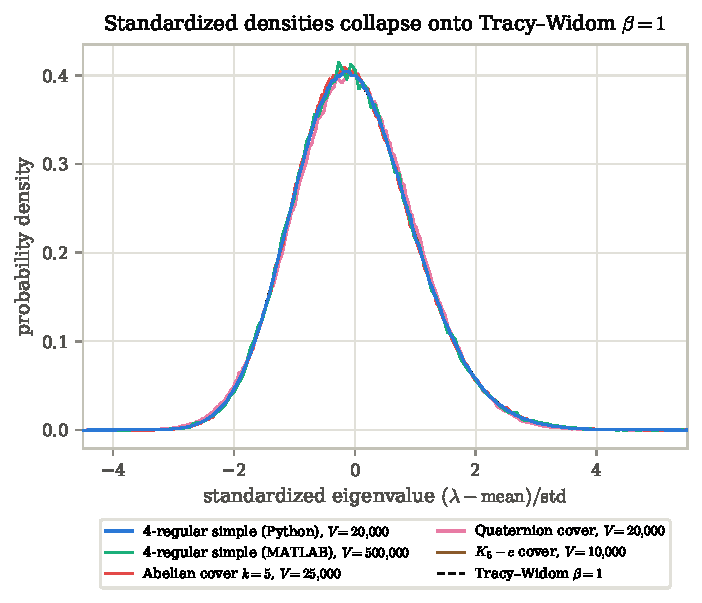
\includegraphics[width=0.75\columnwidth]{images/pdf_universality_across_families.pdf}
\par\end{centering}
\caption{\label{fig:universality}Standardized empirical densities of the
largest datasets from five families overlaid on the standardized $\beta=1$
Tracy-Widom density. The $\beta$ classes are indistinguishable at
this resolution, and are separated by the statistics of Figures \ref{fig:ks_matrix},
\ref{fig:tails}, \ref{fig:ks_classes}, \ref{fig:mass_left}, and
\ref{fig:moments}.}
\end{figure}


\subsection{\label{subsec:amplitudes}The Scale Constants}

Conjecture \ref{conj:symmetry_classes} predicts the scale as well
as the class, and the parameter-free variable of subsection \ref{subsec:statistics}
tests it with the constant $c(4)$ of random $4$-regular graphs and
the base size $n$ as the block dimension. For the character blocks
this rests on the fact that each block $A_{\chi}$ is the adjacency
matrix of the random base graph with its entries rotated by the unimodular
phases $\chi(\sigma_{e})$, a perturbation which does not change the
tree-like local structure or the Kesten-McKay law. The data confirms
the prediction for every family (Figure \ref{fig:scale_location}).
At $n=5000$ the scale ratios are $1.0083\pm0.0006$ for $\mathbb{Z}_{3}$,
$1.0055\pm0.0013$ for $\mathbb{Z}_{5}$, and $0.9901\pm0.0012$ for
$\mathbb{Z}_{4}$, each converging monotonically to $1$, and $1.0052\pm0.0008$
for the quaternion covers, against the constant $c(4)$ with the GSE
normalization $\chi_{4}=2^{-1/6}TW_{4}$ of subsection \ref{subsec:laws}.
Without the factor $2^{-1/6}$ the quaternion ratio would be $0.896$,
and so the data selects the GSE normalization of the Gaussian ensembles,
and the quaternionic block carries the same constant as every other
block. Figure \ref{fig:paramfree_covers} shows the parameter-free
distribution functions against the conjectured laws: the differences
shrink with $n$ in every family, and after the affine fit the Kolmogorov-Smirnov
distances at the largest size are between $0.5\times10^{-3}$ and
$1.2\times10^{-3}$, at the sampling floor. The location coefficients
settle at family dependent constants, $a=-0.35$ for $\mathbb{Z}_{3}$,
$+1.05$ for $\mathbb{Z}_{4}$, $+0.05$ for $\mathbb{Z}_{5}$, and
$-0.77$ for the quaternion covers, each with standard error near
$0.01$, all much smaller than the $4.47$ of the simple graphs.

\begin{figure}[tbp]
\begin{centering}
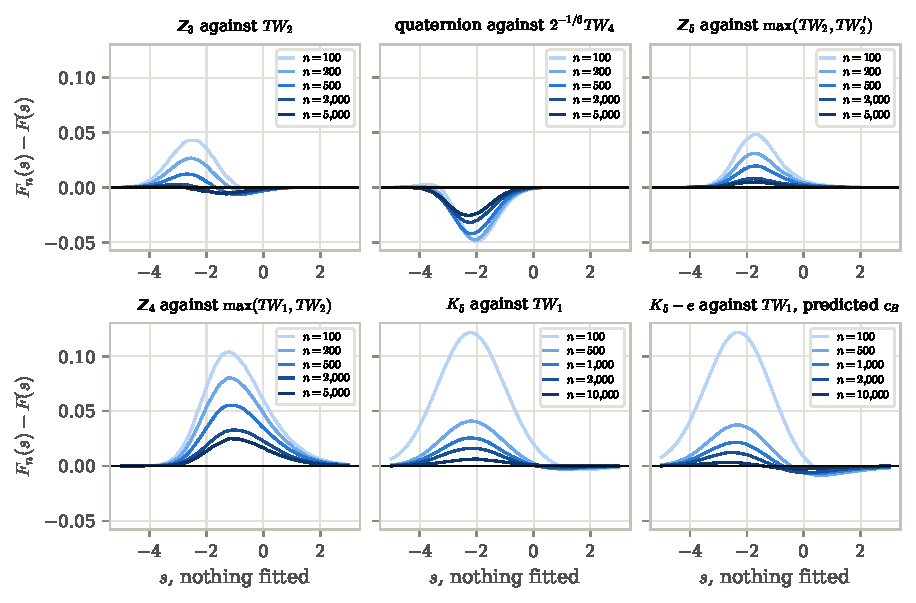
\includegraphics[width=0.95\columnwidth]{images/paramfree_covers.pdf}
\par\end{centering}
\caption{\label{fig:paramfree_covers}Parameter-free comparison of six cover
families with their conjectured laws: $F_{n}(s)-F(s)$, where $F_{n}$
is the empirical distribution function of $s=(\lambda-\rho)N^{2/3}/c$
with the predicted $c$, at five sizes each (lightest: smallest). The
$K_{5}-e$ panel uses the universal cover constant $C_{B}^{-2/3}=0.695228$
of (\ref{eq:edge_constants}). Nothing is fitted.}
\end{figure}


\subsection{\label{subsec:mixed}The Mixed Families and the Maximum Law}

The largest new eigenvalue of a $\mathbb{Z}_{4}$ cover is the maximum
of a GOE class maximum and a GUE class maximum, and that of a $\mathbb{Z}_{5}$
cover is the maximum of two GUE class maxima, and so under Conjectures
\ref{conj:symmetry_classes} and \ref{conj:ramanujan_probabilities}
neither should converge to any single Tracy-Widom law. This is visible
in the raw statistics: the Kolmogorov-Smirnov distance of the standardized
$\mathbb{Z}_{4}$ family to every candidate law grows with $V$, reaching
$1.9\times10^{-2}$ against $\widetilde{TW}_{1}$ at the largest size,
and the $\mathbb{Z}_{5}$ family, nearest $\widetilde{TW}_{1}$ at
moderate sizes, drifts away from it as $V$ grows.

The maximum structure can be tested quantitatively. If the two blocks
of a family fluctuate independently with the same centering $2\sqrt{d-1}$
and the same scale constant, as Conjecture \ref{conj:symmetry_classes}
asserts, then the largest new eigenvalue converges, on the scale $c(d)n^{-2/3}$,
to
\[
M=\max\left(X_{1},X_{2}\right),
\]
where $X_{1},X_{2}$ are independent Tracy-Widom variables of the
appropriate classes, with distribution function $F_{1}F_{2}$ (for
$\mathbb{Z}_{4}$) and $F_{2}^{2}$ (for $\mathbb{Z}_{5}$). After
the affine fit, the Kolmogorov-Smirnov distance of each family to
its maximum law falls with $n$ to $1.2\times10^{-3}$ for $\mathbb{Z}_{4}$
and $0.7\times10^{-3}$ for $\mathbb{Z}_{5}$ at $n=5000$, while
the distances to the pure laws grow (Figure \ref{fig:maxlaw}). Note
that the drift away from the pure laws is invisible at moderate sizes:
up to $n=2000$ the $\mathbb{Z}_{5}$ family is closer in shape to
$TW_{1}$ than to its own maximum law, whose skewness and kurtosis
are close to those of $TW_{1}$, and with $10^{6}$ samples at $V=2500$
the Kolmogorov-Smirnov test accepts $\widetilde{TW}_{1}$ ($p=0.81$),
a caution for experiments at the scale of MNS.

\begin{figure}[tbp]
\begin{centering}
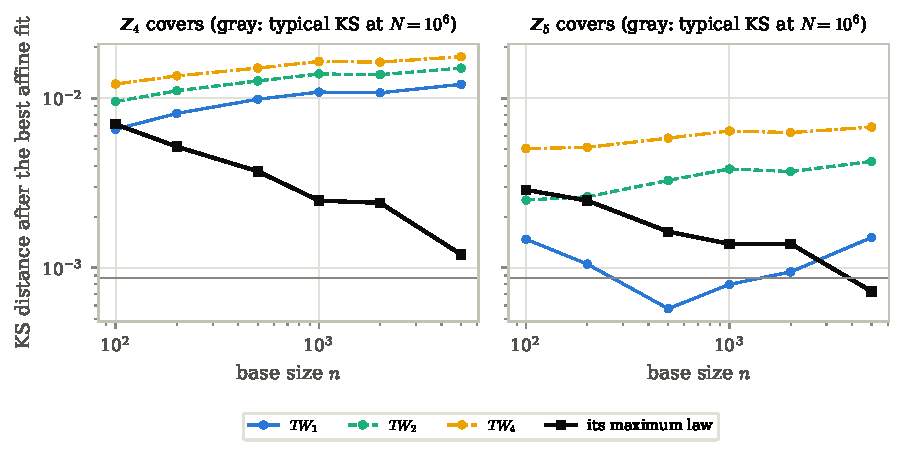
\includegraphics[width=0.95\columnwidth]{images/maximum_law_ks.pdf}
\par\end{centering}
\caption{\label{fig:maxlaw}Kolmogorov-Smirnov distance after the best affine
fit, for the $\mathbb{Z}_{4}$ (left) and $\mathbb{Z}_{5}$ (right)
cover families, to the three Tracy-Widom laws and to the family's
own maximum law, $\max(TW_{1},TW_{2})$ and $\max(TW_{2},TW_{2}')$.
Only the distance to the maximum law falls with $n$.}
\end{figure}

Computing the distribution functions $F_{1}F_{2}$ and $F_{2}^{2}$
numerically gives the predicted constants in Table \ref{tab:predicted_observed}:
the ratio $\left|\mu_{M}\right|/\sigma_{M}$, the mass of $M$ left
of its mean, and the Ramanujan functional $F_{\beta_{1}}(0)F_{\beta_{2}}(0)$.
The $\mathbb{Z}_{5}$ family, whose two blocks have identical marginal
distributions, matches the mass and Ramanujan predictions to three
decimal places at $n=5000$, and the ratio to within $3\times10^{-3}$.
The $\mathbb{Z}_{4}$ family is still drifting at $n=5000$, in each
statistic monotonically toward the predicted value, and the cause
is its location coefficient $a=1.05$, the largest among the covers.
With it, the finite size law (\ref{eq:finite_size_law}) predicts
the $\mathbb{Z}_{4}$ Ramanujan probability $F_{1}F_{2}(a/(c(4)n^{1/3}))=0.82291$
at $n=5000$, against the observed $0.82293$. The maximum structure
is visible at the moment level as well: at $n=5000$ the $\mathbb{Z}_{4}$
skewness and excess kurtosis are $\left(0.570,0.658\right)$ against
the $\max(TW_{1},TW_{2})$ values $\left(0.584,0.670\right)$, and
the $\mathbb{Z}_{5}$ values are $\left(0.320,0.212\right)$ against
$\left(0.329,0.225\right)$, in each case drifting monotonically toward
the prediction (Figure \ref{fig:moment_plane}).

\begin{table}
\begin{centering}
{\footnotesize\setlength{\tabcolsep}{4pt}
\begin{tabular}{|c|c|c|c|c|}
\hline
family & limit law & $g_{V}$ & mass left of mean & $P(\text{Ramanujan})$\tabularnewline
\hline
simple $4$-regular & $TW_{1}$ & $0.9993\ (0.9515)$ & $0.52011\ (0.51965)$ & $0.84352\ (0.83191)$\tabularnewline
\hline
$\mathbb{Z}_{3}$ covers & $TW_{2}$ & $1.9369\ (1.9640)$ & $0.51450\ (0.51502)$ & $0.96793\ (0.96937)$\tabularnewline
\hline
$\mathbb{Z}_{4}$ covers & $\max(TW_{1},TW_{2})$ & $0.8811\ (0.8099)$ & $0.53763\ (0.53895)$ & $0.82293\ (0.80643)$\tabularnewline
\hline
$\mathbb{Z}_{5}$ covers & $\max(TW_{2},TW_{2}')$ & $1.6245\ (1.6219)$ & $0.52122\ (0.52193)$ & $0.94011\ (0.93968)$\tabularnewline
\hline
quaternion covers & $TW_{4}$ & $3.1263\ (3.2061)$ & $0.51094\ (0.51107)$ & $0.99825\ (0.99857)$\tabularnewline
\hline
$K_{5}$ covers & $TW_{1}$ & $0.9551\ (0.9515)$ & $0.51891\ (0.51965)$ & $0.83281\ (0.83191)$\tabularnewline
\hline
$K_{5}-e$ covers & $TW_{1}$ & $0.9387\ (0.9515)$ & $0.51890\ (0.51965)$ & $0.82916\ (0.83191)$\tabularnewline
\hline
$K_{4}-e$ covers & $TW_{1}$ & $0.7326\ (0.9515)$ & $0.52518\ (0.51965)$ & $0.79490\ (0.83191)$\tabularnewline
\hline
\end{tabular}}
\par\end{centering}
\caption{\label{tab:predicted_observed}Observed statistics at the largest
available size of each family against the values predicted by Conjectures
\ref{conj:symmetry_classes}, \ref{conj:ramanujan_probabilities},
and \ref{conj:irregular_base}: the ratio $g_{V}=\left(\rho-\mu_{V}\right)/\sigma_{V}$
of the mean gap to the standard deviation, the mass left of the sample
mean, and the fraction of samples below the Ramanujan threshold $\rho$
($\rho=2\sqrt{3}$ except for the $K_{5}-e$ and $K_{4}-e$ rows, where
$\rho$ is the spectral radius of the universal cover of the base).
Predicted values for the maximum laws were computed numerically from
the Tracy-Widom distributions assuming independent blocks on a common
scale. Each cell shows the observed value with the predicted limit
in parentheses. Observed values are at $V=500{,}000$ (simple), $n=5000$
(abelian and quaternion covers), and $V=10{,}000$ (the fixed base
families). The remaining gaps in the Ramanujan column are the $1/n$
shifts of Table \ref{tab:finite_size}.}
\end{table}

\begin{table}
\begin{centering}
{\footnotesize\setlength{\tabcolsep}{4pt}
\begin{tabular}{|c|c|c|c|c|c|}
\hline
family & size & predicted scale & scale ratio $\gamma$ & location $a$ & KS after affine fit\tabularnewline
\hline
simple $4$-regular & $V=20{,}000$ & $c(4)=0.832683$ & $1.0031\pm0.0003$ & $4.453\pm0.020$ & $0.7\times10^{-3}$\tabularnewline
\hline
simple (legacy) & $V=500{,}000$ & $c(4)$ & $1.0036\pm0.0033$ & $4.30\pm0.37$ & $1.2\times10^{-3}$\tabularnewline
\hline
multigraph & $V=500{,}000$ & $c(4)$ & $0.9992\pm0.0027$ & $-1.31\pm0.34$ & $1.6\times10^{-3}$\tabularnewline
\hline
$\mathbb{Z}_{3}$ covers & $n=5000$ & $c(4)$ & $1.0083\pm0.0006$ & $-0.351\pm0.018$ & $0.8\times10^{-3}$\tabularnewline
\hline
$\mathbb{Z}_{4}$ covers & $n=5000$ & $c(4)$ & $0.9901\pm0.0012$ & $1.022\pm0.026$ & $1.2\times10^{-3}$\tabularnewline
\hline
$\mathbb{Z}_{5}$ covers & $n=5000$ & $c(4)$ & $1.0055\pm0.0013$ & $0.022\pm0.028$ & $0.7\times10^{-3}$\tabularnewline
\hline
quaternion covers & $n=5000$ & $c(4)$, $\chi_{4}=2^{-1/6}TW_{4}$ & $1.0052\pm0.0008$ & $-0.742\pm0.026$ & $0.5\times10^{-3}$\tabularnewline
\hline
$K_{5}$ covers & $V=10{,}000$ & $c(4)$ & $1.0091\pm0.0003$ & $0.073\pm0.012$ & $0.7\times10^{-3}$\tabularnewline
\hline
$K_{5}-e$ covers & $V=10{,}000$ & $C_{B}^{-2/3}=0.695228$ & $1.0119\pm0.0003$ & $-0.233\pm0.014$ & $0.6\times10^{-3}$\tabularnewline
\hline
$K_{4}-e$ covers & $V=10{,}000$ & $C_{B}^{-2/3}=0.212519$ & $1.0441\pm0.0009$ & $-0.922\pm0.007$ & $2.8\times10^{-3}$\tabularnewline
\hline
\end{tabular}}
\par\end{centering}
\caption{\label{tab:finite_size}The finite size law (\ref{eq:finite_size_law})
at the largest size of each family: the predicted scale, the scale
ratio, the location coefficient, and the Kolmogorov-Smirnov distance
of the sample to its conjectured law after the affine fit, with standard
errors from ten batches. The typical distance of a sample from its
own law is $0.4\times10^{-3}$ at $5\times10^{6}$ samples, $0.9\times10^{-3}$
at $10^{6}$, and $2.7\times10^{-3}$ at $10^{5}$.}
\end{table}

The Ramanujan column of Table \ref{tab:predicted_observed} is the
experimental form of Conjecture \ref{conj:ramanujan_probabilities}.
Each family approaches the product $\prod F_{\beta}(0)$ over its
blocks: one GUE block gives $F_{2}(0)=0.96937\dots$ for $\mathbb{Z}_{3}$,
two give $F_{2}(0)^{2}=0.93968\dots$ for $\mathbb{Z}_{5}$, matched
by the observed $0.94011$ at $n=5000$, the mixed $\mathbb{Z}_{4}$
product $F_{1}(0)F_{2}(0)=0.80643\dots$ is approached from above
through $0.82293$, and the quaternion block gives $F_{4}(0)=0.99857\dots$
against the observed $0.99825$. The residual gaps are the location
shifts: evaluating each law at its shifted point $a/(cN^{1/3})$ reproduces
every observed Ramanujan fraction in the table to within $3\times10^{-4}$,
and to within $6\times10^{-4}$ for $K_{4}-e$.
Figure \ref{fig:prob_ramanujan} shows the full curves, and Figure
\ref{fig:ratio} the underlying ratios $g_{V}$, each family flattening
onto the ratio of its own limit law. In particular the limiting probability
of being Ramanujan is not one number but a representation theoretic
invariant of the family, always strictly between $0$ and $1$.

\begin{figure}[tbp]
\begin{centering}
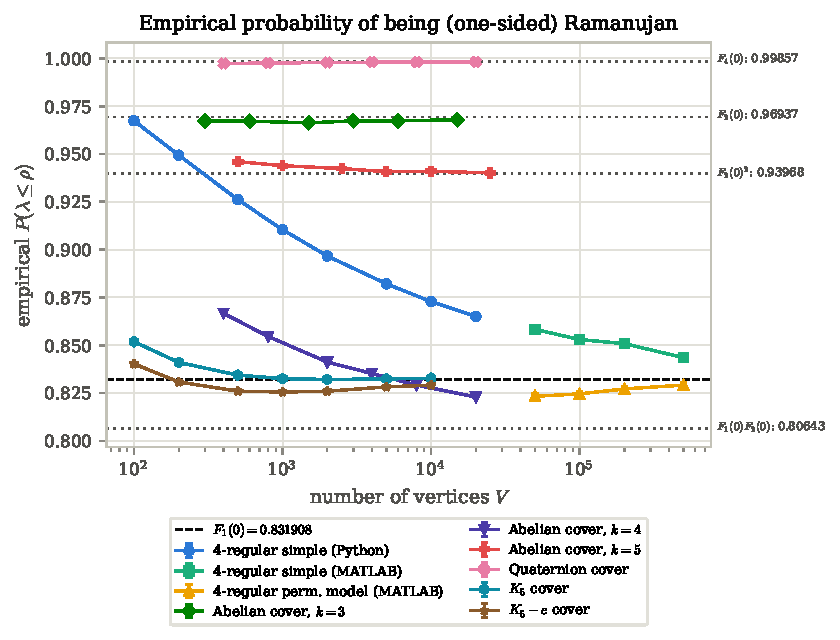
\includegraphics[width=0.8\columnwidth]{images/prob_ramanujan_vs_size_all_families.pdf}
\par\end{centering}
\caption{\label{fig:prob_ramanujan}Empirical $P\left(\lambda\leq\rho\right)$
against $V$ for all families, where $\rho$ is the family's Ramanujan
threshold, with the limit $F_{1}(0)=0.8319081\dots$ for the $\beta=1$
families. Each cover family approaches the product of Tracy-Widom
functionals of Conjecture \ref{conj:ramanujan_probabilities} listed
in Table \ref{tab:predicted_observed}.}
\end{figure}

\begin{figure}[tbp]
\begin{centering}
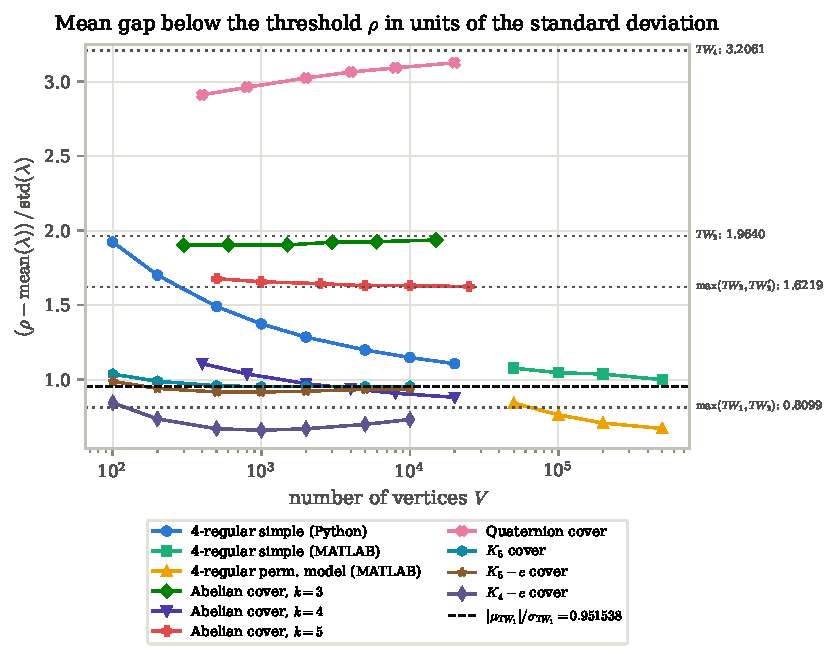
\includegraphics[width=0.8\columnwidth]{images/ratio_mean_gap_over_std_vs_size_all_families.pdf}
\par\end{centering}
\caption{\label{fig:ratio}The ratio $g_{V}=\left(\rho-\mu_{V}\right)/\sigma_{V}$
against $V$ for all families, where $\rho$ is the family's Ramanujan
threshold, with the $\beta=1$ reference $\left|\mu_{TW_{1}}\right|/\sigma_{TW_{1}}=0.951537\dots$
dashed. MNS conjectured this ratio tends to $0$, however each family
plateaus at the ratio of its own limit law: $1.96$ for $\mathbb{Z}_{3}$,
$1.62$ for $\mathbb{Z}_{5}$, $3.21$ for quaternion covers, and the
$\beta=1$ reference for the regular and fixed base families.}
\end{figure}


\section{\label{sec:irregular}Covers of a Fixed Base Graph}

We now fix the base graph and let only the cover vary, testing three
bases: the complete graph $K_{5}$, whose covers are $4$-regular and
calibrate the fixed base model against section \ref{sec:regular},
the irregular graph $K_{5}-e$, and the cycle rank two graph $K_{4}-e$
of subsection \ref{subsec:k4e}. Nothing in Conjecture \ref{conj:irregular_base}
requires the base graph to be regular, and in the irregular case nothing
is proven: the largest new eigenvalue should concentrate at the spectral
radius $\rho(B)$ of the universal cover, an algebraic number lying
between $2\sqrt{\delta-1}$ and $2\sqrt{\Delta-1}$, where $\delta$
and $\Delta$ are the minimum and maximum degrees of $B$, with $TW_{1}$
fluctuations on the scale $(C_{B}nk)^{-2/3}$ and limiting Ramanujan
probability $F_{1}(0)$, universally in the base graph. The threshold
$\rho(B)$ is also the benchmark of the $X$-Ramanujan property of
Mohanty and O'Donnell \cite{MohantyODonnell2020}, who construct infinite
families of finite graphs whose second eigenvalue is at most the spectral
radius of a fixed infinite cover. It is the right benchmark: by the
generalized Alon-Boppana theorems of Friedman and Tillich \cite{FriedmanTillich2005},
no infinite family of graphs sharing the universal cover of $B$ has
second eigenvalue asymptotically below $\rho(B)$, and Hoory \cite{Hoory2005}
bounds $\rho(B)$ itself below by $2\sqrt{\bar{d}-1}$, where $\bar{d}$
is the average degree of $B$. Random bipartite biregular graphs, whose limiting
tree is not regular either, satisfy an Alon type theorem as well \cite{BritoDumitriuHarris2022}.

The main base is $K_{5}-e$, the complete graph on five vertices minus
an edge, one of the smallest irregular base graphs of minimum degree
three, with eigenvalues $1+\sqrt{7}=3.6457\dots$, $0$, $-1$, $-1$,
and $1-\sqrt{7}$. Since the largest old eigenvalue exceeds $\rho(K_{5}-e)$,
the largest new eigenvalue of a cover is not even its second largest
eigenvalue, so that the exact removal of the lifted base spectrum
matters. By a result of McKay \cite{McKay2023}, $\rho(K_{5}-e)$
is the largest zero of
\[
x^{14}-20x^{12}+122x^{10}-152x^{8}-1295x^{6}+4540x^{4}-5948x^{2}-2000,
\]
an irreducible polynomial whose roots admit no expression in radicals,
giving
\[
\rho(K_{5}-e)=3.26287646593635862827\dots,
\]
which we re-derived and verified independently, and which also follows
from the variational formula of Garza-Vargas and Kulkarni \cite{GarzaVargasKulkarni2023}.
Note the contrast with the regular case, where $\rho=2\sqrt{d-1}$:
for a general base even the centering of the conjectured law is a
non-trivial algebraic quantity (see \cite{AngelFriedmanHoory2015,GarzaVargasKulkarni2023,McKay2023}
on computing $\rho$, and \cite{CrawfordMarchetteMaxwellMendelson2023}
for related spectral experiments on structured random graphs), and
so is the scale constant $C_{B}$ of (\ref{eq:edge_constants}).

\subsection{\label{subsec:bulk_law}The Bulk Law}

We sampled the $K_{5}$ and $K_{5}-e$ families at the scale of the
strongest regular graph data: $5\times10^{6}$ independent uniform
covers per size, at cover degrees $20\leq k\leq2000$, giving graphs
on $V=5k$ between $100$ and $10{,}000$ vertices. The covers of $K_{5}$
are $4$-regular graphs with Ramanujan threshold $2\sqrt{3}$, of
a different fine structure than the permutation model, since the vertex
set carries a fixed partition into five independent fibers with edges
only between fibers adjacent in $K_{5}$, and so they test whether
the limit law and its constants depend on anything beyond the degree.
The covers of $K_{5}-e$ test Conjecture \ref{conj:irregular_base}
where no theorem reaches, around the algebraic centering $\rho(K_{5}-e)$
and on the scale set by the new constant $C_{K_{5}-e}$.

\begin{figure}[tbp]
\begin{centering}
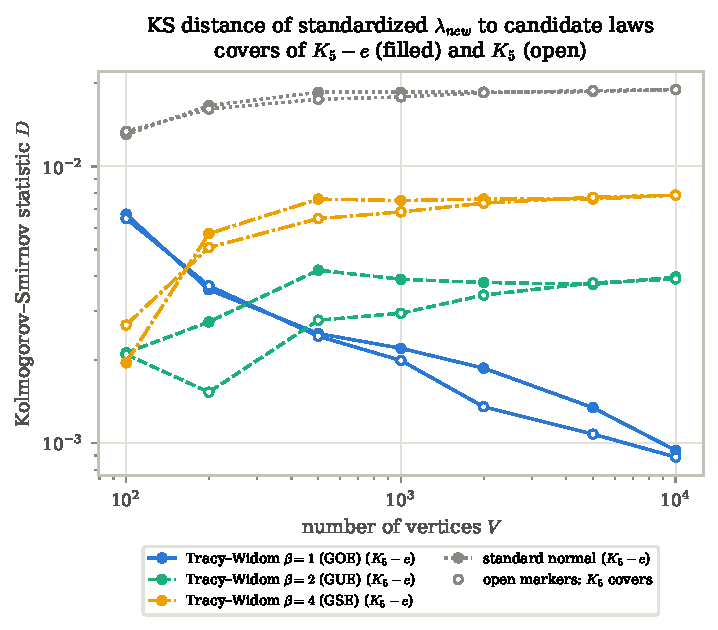
\includegraphics[width=0.75\columnwidth]{images/ks_statistic_vs_size_k5_covers.pdf}
\par\end{centering}
\caption{\label{fig:ks_k5}Kolmogorov-Smirnov distance of the standardized
largest new eigenvalue to the four candidate laws for covers of $K_{5}-e$
(filled markers, standardized around $\rho(K_{5}-e)$) and of $K_{5}$
(open markers), $5\times10^{6}$ samples per size. For both families
only the distance to $\beta=1$ keeps falling.}
\end{figure}

Figure \ref{fig:ks_k5} shows the outcome of the distributional test.
For both families the Kolmogorov-Smirnov distance to $\widetilde{TW}_{1}$
falls monotonically with $V$, reaching $8.9\times10^{-4}$ for $K_{5}$
and $9.4\times10^{-4}$ for $K_{5}-e$ at $V=10{,}000$, a small multiple
of the sampling floor and equal to the simple $4$-regular family's
distance at the same size, while the distances to the other laws
stall or grow, ending at $4.0\times10^{-3}$ ($\widetilde{TW}_{2}$),
$7.9\times10^{-3}$ ($\widetilde{TW}_{4}$), and $1.9\times10^{-2}$
(normal) for $K_{5}-e$. A two sample comparison is sharper still:
the Kolmogorov-Smirnov distance between the standardized simple and
$K_{5}$ samples at $V=10{,}000$ is $3.7\times10^{-4}$ ($p=0.88$),
while each lies $8.9\times10^{-4}$ from $\widetilde{TW}_{1}$ ($p\approx10^{-3}$),
and so at $10^{7}$ combined samples the two models are statistically
indistinguishable from one another in shape while both still differ
measurably from the limit. At small sizes the families are well separated
($p=2\times10^{-15}$ at $V=100$), merging from $V\approx5000$ on.
Figure \ref{fig:pdf_k5e} shows the standardized density of the largest
$K_{5}-e$ dataset, and Figure \ref{fig:qq_k5e} the corresponding
quantile plot. The mass left of the mean reaches $0.51891$ ($K_{5}$)
and $0.51890$ ($K_{5}-e$) against the $TW_{1}$ value $0.519652$,
on the same convergence path as the simple family at equal sizes,
and the ratio $g_{V}$ reaches $0.9551$ and $0.9387$ against the
$TW_{1}$ ratio $\left|\mu_{TW_{1}}\right|/\sigma_{TW_{1}}$ (Figure
\ref{fig:ratio}). The local exponents of the mean gap and standard
deviation descend to $-0.673$ and $-0.676$ for $K_{5}$ and $-0.670$
and $-0.678$ for $K_{5}-e$ over the last pair of sizes, approaching
$-2/3$ as for the regular families (Figure \ref{fig:local_exponent}).
The empirical Ramanujan probabilities at $V=10{,}000$ are
\[
P\left(\lambda_{\mathrm{new}}\leq2\sqrt{3}\right)=0.83281,\ \ \ P\left(\lambda_{\mathrm{new}}\leq\rho(K_{5}-e)\right)=0.82916,
\]
against the conjectured $F_{1}(0)=0.8319081\dots$ (Table \ref{tab:predicted_observed}).
Every statistic selects the $\beta=1$ class, as the reality of the
standard representation predicts, and for $K_{5}-e$ it does so around
a centering which is not $2\sqrt{d-1}$ for any $d$.

\begin{figure}[tbp]
\begin{centering}
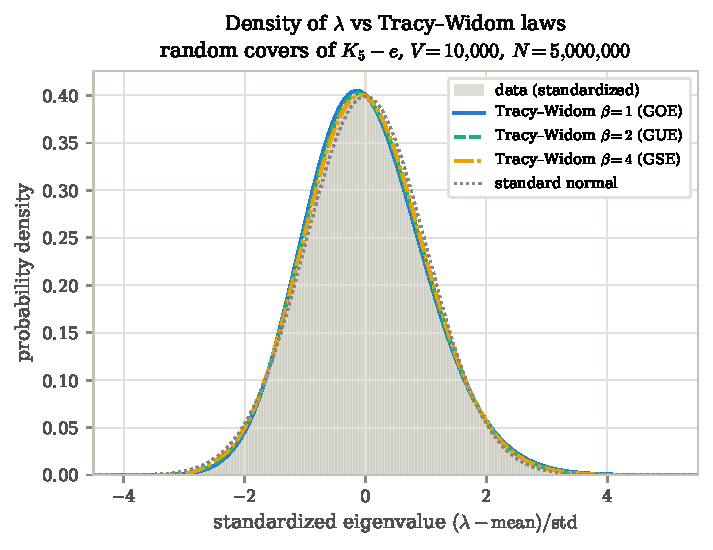
\includegraphics[width=0.7\columnwidth]{images/pdf_vs_tracywidom_k5_minus_edge_V10000_N5000000.pdf}
\par\end{centering}
\caption{\label{fig:pdf_k5e}Standardized empirical density of the largest
new eigenvalue over $5\times10^{6}$ random covers of $K_{5}-e$ at
$V=10{,}000$, against the standardized Tracy-Widom densities and
the standard normal.}
\end{figure}

\begin{figure}[tbp]
\begin{centering}
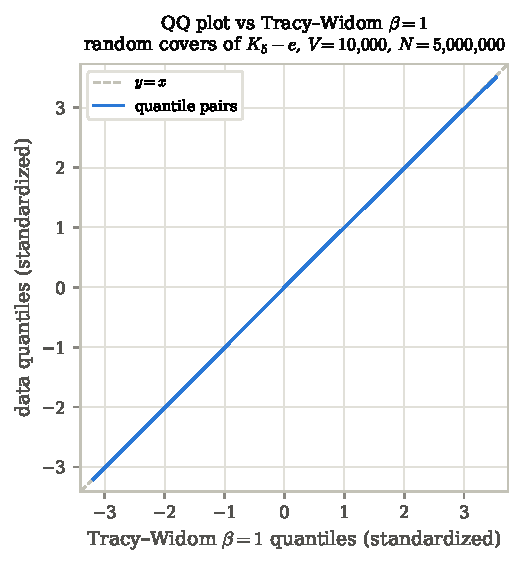
\includegraphics[width=0.6\columnwidth]{images/qq_vs_tracywidom1_k5_minus_edge_V10000_N5000000.pdf}
\par\end{centering}
\caption{\label{fig:qq_k5e}Quantile-quantile plot of the largest $K_{5}-e$
dataset against $\widetilde{TW}_{1}$, probability range $10^{-4}$
to $0.999$: the bulk of the law around the algebraic centering $\rho(K_{5}-e)$
is Tracy-Widom at quantile resolution.}
\end{figure}

The amplitudes are the sharpest test of Conjecture \ref{conj:irregular_base},
since for $K_{5}-e$ the predicted constant $C_{B}^{-2/3}=0.695228\dots$
of (\ref{eq:edge_constants}) was computed from the universal cover
alone, with no reference to the data. The fitted amplitudes $\gamma_{V}c(4)$
descend through $0.7209$, $0.7085$, and $0.7035$ at $V=2000$, $5000$,
and $10{,}000$, and a fit $c+bV^{-2/3}$ over $V\geq1000$ or $V\geq2000$
extrapolates to $0.6943$ to $0.6949$, within $0.15\%$ of the prediction
(Figure \ref{fig:irregular_amplitude}). The same fits for $K_{5}$
give $0.8315$ to $0.8319$ against $c(4)=0.832683$, and so the amplitude
constant for covers of $K_{5}$ is the regular graph constant $c(4)$
itself, in the convention with $V$ the cover size, as the Kesten-McKay
law of $\mu_{K_{5}}$ requires. The speed of convergence differs,
however: the $K_{5}$ family sits within $10^{-3}$ of the limiting
Ramanujan probability from $V=1000$ onward ($0.83258$ at $V=1000$),
while the simple $4$-regular series is still at $0.87282$ at $V=10{,}000$,
and the $K_{5}$ ratio $g_{V}$ is already $0.9522$ at $V=1000$ against
the simple series' $1.148$ at ten times that size. The difference
lies in the location coefficient, which is $a\approx0.03$ for $K_{5}$
against $4.47$ for the simple graphs (Table \ref{tab:finite_size}),
and not in the scale, which for $K_{5}$ converges if anything more
slowly, with scale ratio $1.046$ at $V=1000$ against $1.027$. The
Ramanujan probability does not see the scale, only the shift.

\begin{figure}[tbp]
\begin{centering}
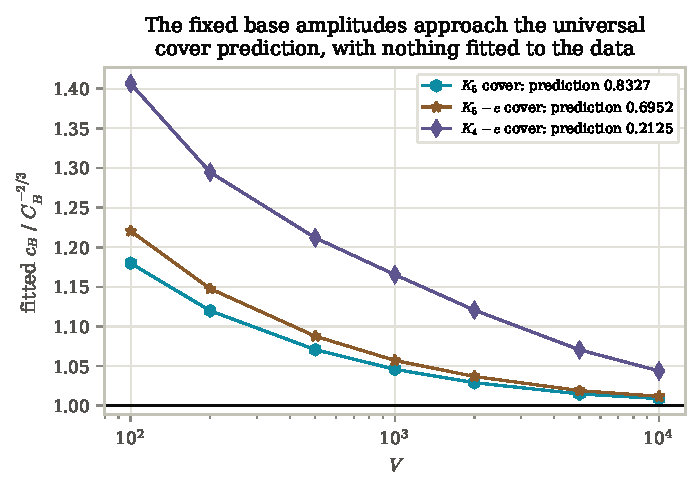
\includegraphics[width=0.7\columnwidth]{images/irregular_amplitude_vs_prediction.pdf}
\par\end{centering}
\caption{\label{fig:irregular_amplitude}The fitted amplitudes of the three
fixed base families over the universal cover predictions $C_{B}^{-2/3}$
of (\ref{eq:edge_constants}), none of which was fitted to the data.
$K_{5}$ and $K_{5}-e$ converge to $1$ together, while $K_{4}-e$,
whose square root regime is narrow, converges more slowly.}
\end{figure}

\subsection{\label{subsec:defects}Localized Defects and the Far Tails}

The third and fourth moments tell a different story, and the accounting
is instructive. The excess kurtosis of the $K_{5}-e$ family grows
with $V$, from $0.26$ at $V=100$ to $2.52$ at $V=10{,}000$ against
the $TW_{1}$ value $0.165$, and its skewness drifts upward through
$0.361$ against $0.293$, while the same statistics for $K_{5}$ are
$0.28$ and $0.292$. Figure \ref{fig:tail_k5} locates the cause
in a thin tail of far outliers, at frequencies near $10^{-5}$: at
$V=10{,}000$ a fraction $9\times10^{-6}$ of the $K_{5}-e$ samples
lie above $\rho+10\sigma_{V}$, while the extreme sample of the simple
$4$-regular family sits only $9$ standard deviations out. These
outliers are the tangles of \cite{Friedman2008} made visible sample
by sample, and they admit a complete quantitative description, one
half of which we can prove. For regular bases, Addario-Berry and Griffiths
\cite{AddarioBerryGriffiths2010} showed that large new eigenvalues
of random lifts are caused by small induced subgraphs, up to a constant
factor, and the propositions below make this exact for the rate and
the location of each defect.

Note that every subgraph of a cover projects to the base graph by
a locally injective map, since distinct neighbors of a vertex of a
cover lie over distinct neighbors of its projection. With this in
mind, fix a connected graph $H$ of minimum degree at least two admitting
a locally injective map, an \emph{immersion}, $\varphi:H\rightarrow B$,
and write $r(H)=e(H)-v(H)+1$ for its cycle rank. Let $H^{*}$ be
the infinite graph obtained from $H$ by attaching, at each vertex
$x$ of $H$ and each neighbor of $\varphi(x)$ not used by an edge
of $H$ at $x$, the corresponding branch of the universal cover of
$B$, and define the \emph{defect eigenvalue}
\[
\lambda_{B}(H)=\left\Vert A_{H^{*}}\right\Vert ,
\]
the spectral norm of the adjacency operator of $H^{*}$, maximized
over the locally injective maps $\varphi$ when there are several.
When $B$ is a bouquet, $H^{*}$ is the tree extension used by Dong
and McKenzie \cite{DongMcKenzie2026} in their proof that every sequence
$d\geq\mu_{2}\geq\cdots\geq\mu_{k}\geq2\sqrt{d-1}$ is a limit of
top eigenvalues of $d$-regular graphs. Deep inside any branch, $H^{*}$
contains arbitrarily large balls of the universal cover, and so $\lambda_{B}(H)\geq\rho(B)$
always, and when the inequality is strict we say that $H$ \emph{binds}
an eigenvalue above $\rho(B)$. When it binds, $\lambda_{B}(H)$ lies
above the essential spectrum, since removing finitely many vertices
from $H^{*}$ leaves a union of branches, and $\lambda_{B}(H)$ is
computable to any precision from the branch values (\ref{eq:branch_recursion})
at real $\lambda>\rho(B)$: each attached branch contributes its value
to the diagonal, and $\lambda_{B}(H)$ is the largest $\lambda$ with
$\lambda_{\max}\left(A_{H}+D(\lambda)\right)=\lambda$, where $D(\lambda)$
is the diagonal matrix of attached branch values (for eigenvalues
of graphs with attached infinite tails see also \cite{Golinskii2016}).
Figure \ref{fig:defect_shapes} shows the leading defects of our families.
Two elementary facts organize the far tails: copies of $H$ appear
in a random cover at a polynomial rate governed by the cycle rank,
and any copy forces a new eigenvalue near $\lambda_{B}(H)$.

\begin{figure}[tbp]
\begin{centering}
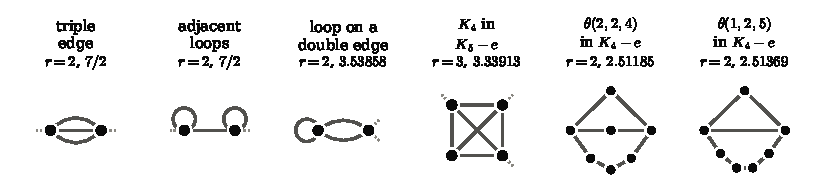
\includegraphics[width=0.98\columnwidth]{images/defect_shapes.pdf}
\par\end{centering}
\caption{\label{fig:defect_shapes}The leading defects, with their cycle ranks
$r$ and defect eigenvalues $\lambda_{B}(H)$: the three binding defects
of cycle rank two of the permutation multigraph (subsection \ref{subsec:multigraph}),
$K_{4}$ immersed in $K_{5}-e$ (in $K_{5}$ it has a fourth attached
branch and binds at $7/2$), and the two shortest binding generalized
thetas of $K_{4}-e$ (subsection \ref{subsec:k4e}, branches not drawn).
Dashed stubs are attached branches of the universal cover.}
\end{figure}

\begin{prop}
\label{prop:defect_counting}Let $B$ be a connected base graph, let
$H$ be a connected graph of minimum degree at least two admitting
a locally injective map to $B$, and let $X_{H}$ be the number of
subgraphs of a uniformly random degree $k$ cover $H_{k}$ of $B$
isomorphic to $H$. Then
\[
E\left[X_{H}\right]=c_{H}k^{1-r(H)}\left(1+O\left(k^{-1}\right)\right),\ \ \ c_{H}=\frac{J(H,B)}{\left|\mathrm{Aut}(H)\right|},
\]
where $J(H,B)$ is the number of locally injective homomorphisms from
$H$ to $B$, and, when $r(H)\geq2$,
\[
P\left(X_{H}\geq1\right)=c_{H}k^{1-r(H)}\left(1+o\left(1\right)\right).
\]
\end{prop}
\begin{proof}
Suppose first that $B$ is simple, as are all of our fixed bases,
since loops and multiple edges require only notational changes. Copies
of $H$ in the cover correspond to pairs consisting of a locally
injective homomorphism $\psi:H\rightarrow B$ and a lift of $\psi$,
with each copy counted $\left|\mathrm{Aut}(H)\right|$ times. Fix
$\psi$, and choose for each vertex of $H$ a lift in the fiber over
its image, injectively within each fiber, which can be done in $k^{v(H)}\left(1+O(k^{-1})\right)$
ways. The chosen vertices span a copy of $H$ exactly when, for each
edge $e$ of $B$, the permutation $\sigma_{e}$ maps every specified
source to its specified target. If $m_{e}$ edges of $H$ lie over
$e$, then the sources are distinct and the targets are distinct,
by fiber injectivity and the local injectivity of $\psi$, and so
this event has probability $\left(k-m_{e}\right)!/k!=k^{-m_{e}}\left(1+O(k^{-1})\right)$,
independently across the edges of $B$. Multiplying and summing over
$\psi$ gives the expectation, since $v(H)-e(H)=1-r(H)$.

For the probability, we have that $E[X_{H}^{2}]=E[X_{H}]+E[Y]$, where
$Y$ counts ordered pairs of distinct copies. The union of two distinct
copies is either disconnected, and such pairs contribute $c_{H}^{2}k^{2-2r}\left(1+O(k^{-1})\right)$
by the computation above, or connected of cycle rank at least $r+1$:
if two distinct copies overlap, their intersection is a proper subgraph
$F$ of $H$, and $r(U)=2r(H)-1-r(F)+q$ for the union $U$, where
$q$ is the number of components of $F$ and $r(F)=e(F)-v(F)+q$,
so it suffices that $r(F)\leq r(H)-2+q$. For connected $F$, with
$q=1$, this says $r(F)\leq r(H)-1$, which holds since a proper connected
subgraph of a graph of minimum degree two has strictly smaller cycle
rank: a path leaving the subgraph cannot terminate, and closes an
independent cycle whether it returns to the subgraph or to itself.
For disconnected $F$, with $q\geq2$, it follows from $r(F)\leq r(H)$,
since the cycle spaces of disjoint subgraphs embed independently into
that of $H$. Each connected union type of cycle rank at least $r+1$
contributes $O(k^{-r})$, and there are finitely many, and so $E[X_{H}^{2}]=E[X_{H}]\left(1+o(1)\right)+E[X_{H}]^{2}\left(1+o(1)\right)$.
The claim follows from $P(X_{H}\geq1)\geq E[X_{H}]^{2}/E[X_{H}^{2}]$
and $P(X_{H}\geq1)\leq E[X_{H}]$.
\end{proof}
The second fact is that every occurrence produces its eigenvalue.
\begin{prop}
\label{prop:defect_eigenvalue}In the setting of Proposition \ref{prop:defect_counting},
suppose that $r(H)\geq2$ and $\lambda_{B}(H)>\rho(B)$. Then for
every $\epsilon>0$ there is a constant $c=c(B,H,\epsilon)>0$ such
that for all $k$ sufficiently large,
\[
P\left(\lambda_{\mathrm{new}}(H_{k})\geq\lambda_{B}(H)-\epsilon\right)\geq c\,k^{1-r(H)}.
\]
\end{prop}
\begin{proof}
Let $H_{\ell}^{*}$ denote the truncation of $H^{*}$ at depth $\ell$
from $H$. Since $H^{*}$ is connected and locally finite, $\lambda_{\max}(H_{\ell}^{*})$
increases to $\left\Vert A_{H^{*}}\right\Vert $ as $\ell\rightarrow\infty$,
and so we may fix $\ell$ with $\lambda_{\max}(H_{\ell}^{*})>\lambda_{B}(H)-\epsilon/2$.
Let $u\geq0$ be the Perron eigenvector of $H_{\ell}^{*}$ with $\left\Vert u\right\Vert =1$,
supported on $N=N(\ell)$ vertices. Call a copy of $H$ in the cover
\emph{clean} if the depth $\ell$ neighborhood of its vertex set is
isomorphic, over $B$, to $H_{\ell}^{*}$. A copy which is not clean
lies in a connected subgraph of the cover of size $O_{\ell}(1)$ and
cycle rank at least $r(H)+1$, since any deviation of the neighborhood
from $H_{\ell}^{*}$ closes an additional independent cycle within
distance $\ell$, and the expected number of these is $O_{\ell}(k^{-r(H)})$
by the computation of Proposition \ref{prop:defect_counting}, and
so with probability at least $c_{H}k^{1-r(H)}\left(1+o(1)\right)$
the cover contains a clean copy.

Given a clean copy, transplant $u$ onto its neighborhood. The subspace
of functions which are constant on every fiber is invariant under
the adjacency matrix $A$ of the cover, its spectrum on this subspace
is the spectrum of $B$, and its spectrum on the orthogonal complement
is exactly the new spectrum. Writing $P$ for the orthogonal projection
onto the fiber constant functions, each fiber meets the support of
$u$ in at most $N$ vertices, and so by the Cauchy-Schwarz inequality
\[
\left\Vert Pu\right\Vert ^{2}=\sum_{b\in V(B)}\frac{1}{k}\left(\sum_{x\in\pi^{-1}(b)}u(x)\right)^{2}\leq\frac{N}{k}.
\]
Set $w=u-Pu$, a vector in the new subspace with $\left\Vert w\right\Vert ^{2}\geq1-N/k$.
Since $u\geq0$ and the neighborhood of the clean copy contains $H_{\ell}^{*}$
as a subgraph, we have that $\left\langle u,Au\right\rangle \geq\lambda_{\max}(H_{\ell}^{*})$,
and since $\left\Vert A\right\Vert $ is at most the maximum degree
of $B$,
\[
\lambda_{\mathrm{new}}(H_{k})\geq\frac{\left\langle w,Aw\right\rangle }{\left\Vert w\right\Vert ^{2}}\geq\left\langle u,Au\right\rangle -3\left\Vert A\right\Vert \left\Vert Pu\right\Vert \geq\lambda_{\max}(H_{\ell}^{*})-O_{\ell}\left(k^{-1/2}\right),
\]
whose right hand side is positive and exceeds $\lambda_{B}(H)-\epsilon$
for $k$ large, and the result follows.
\end{proof}
One family of defects is degenerate. A graph which is itself a cover
of $B$, beginning with $B$ under the identity, saturates every direction
at every vertex, and so a copy of it is a full connected component,
with defect eigenvalue its own Perron eigenvalue: its occurrence disconnects
the cover, and by removal by value (subsection \ref{subsec:dataset})
the pipeline records instead the largest remaining eigenvalue outside
the base spectrum. We exclude covers of $B$ from the defect catalogue
and from the minimum in the conjecture below, and by Proposition \ref{prop:defect_counting}
the disconnected covers have probability $O(k^{1-r(B)})$. We believe
that the remaining defects account for the entire polynomial tail,
and conjecture the matching upper bound.
\begin{conjecture}
\label{conj:defect_completeness}Let $B$ be a connected base graph
of cycle rank at least two, and let $H_{k}$ be a uniformly random
degree $k$ cover of $B$, conditioned on connectedness. Then for every
$\epsilon>0$,
\[
P\left(\lambda_{\mathrm{new}}(H_{k})>\rho(B)+\epsilon\right)=k^{1-r(\epsilon)+o(1)},
\]
where
\[
r(\epsilon)=\min\left\{ r(H):\ H\text{ immerses in }B\text{ and is not a cover of }B,\ \lambda_{B}(H)>\rho(B)+\epsilon\right\} ,
\]
and where the probability is smaller than every power of $k$ when
no such $H$ exists.
\end{conjecture}
For regular Ramanujan bases, Conjecture \ref{conj:defect_completeness}
is essentially the theorem of Friedman and Kohler \cite{FriedmanKohler2014,FriedmanKohler2019},
and the coexistence of a Tracy-Widom bulk with a thin family of localized
outliers is the picture proven at the sparse Erd\H{o}s-R\'{e}nyi edge
\cite{AltDucatezKnowles2021,AltDucatezKnowles2023,AltDucatezKnowles2024,HiesmayrMcKenzie2025},
and for sparse Wigner matrices the outliers are likewise produced
by localized defects \cite{TikhomirovYoussef2021}. The eigenvectors
near a Tracy-Widom edge are delocalized, and for random regular graphs
they are locally Gaussian waves \cite{HeHuangYau2025}, as they are
in small spectral windows for random lifts \cite{DemboMcKenzie2026},
so that the two populations differ in their eigenvectors as well as
in their eigenvalues. The mechanism is not tied to randomness: Alon,
Ganguly, and Srivastava \cite{AlonGangulySrivastava2021} construct
regular graphs of high girth whose top eigenvectors are fully localized
on small vertex sets, and every value in $[2\sqrt{d-1},d]$ is a limit
point of second eigenvalues of $d$-regular graphs \cite{AlonWei2023,DongMcKenzie2026}.
Proposition \ref{prop:defect_eigenvalue} is the elementary half in
general. Together with the fluctuation conjecture, the defect picture
determines exactly which statistics converge.
\begin{cor}
\label{cor:moment_divergence}Assume the scaling of Conjecture \ref{conj:irregular_base},
and suppose that some $H$ immersing in $B$, not a cover of $B$,
has $\lambda_{B}(H)>\rho(B)$, with $r^{*}\geq2$ the least cycle
rank of such an $H$. Then the $p^{th}$ absolute moment of $\left(\lambda_{\mathrm{new}}(H_{k})-\rho(B)\right)k^{2/3}$
diverges as $k\rightarrow\infty$ for every $p>3\left(r^{*}-1\right)/2$.
\end{cor}
To see this, note that a defect at fixed height $\Delta=\lambda_{B}(H)-\rho(B)$
sits at $\Delta/\sigma_{k}\asymp\Delta k^{2/3}$ standardized units
above the mean, and occurs with probability $\asymp k^{1-r^{*}}$
by Propositions \ref{prop:defect_counting} and \ref{prop:defect_eigenvalue},
and so contributes to the $p^{th}$ standardized moment at order
\begin{equation}
k^{1-r^{*}}\left(\Delta k^{2/3}\right)^{p}\asymp k^{1-r^{*}+\frac{2p}{3}},\label{eq:moment_exponent}
\end{equation}
which diverges exactly when $p>3\left(r^{*}-1\right)/2$. Under Conjecture
\ref{conj:defect_completeness}, holding uniformly down to the fluctuation
scale, the moments below the threshold converge instead to those of
the limit law. Equation (\ref{eq:moment_exponent}) organizes every
moment anomaly in this paper. For the permutation multigraph model
and for $K_{4}-e$, where $r^{*}=2$, the variance itself is eventually
dominated by the defect band, growing relative to the bulk like $k^{1/3}$,
and at the bulk scale the skewness diverges like $k$ and the kurtosis
like $k^{5/3}$, so that the raw moments of these families are the
most contaminated in the dataset, which is what subsection \ref{subsec:multigraph}
observed, and the raw ratio $g_{V}$ of subsection \ref{subsec:k4e}
must eventually turn around and decrease, with only its trimmed version
converging to the $TW_{1}$ ratio. For $K_{5}-e$ and $K_{5}$, where
$r^{*}=3$, the variance is safe, the kurtosis diverges like $k^{2/3}$,
matching the observed growth, and $p=3$ is exactly critical: the
defects add a constant, non-vanishing offset to the skewness, which
is why the $K_{5}-e$ skewness settles near $0.36$ rather than at
the Tracy-Widom value $0.293$, while for $K_{5}$ the constant is
too small to resolve. Every quantile level statistic is immune, since
the total defect mass vanishes: the Kolmogorov-Smirnov distance moves
by at most the tail mass and the Ramanujan probability by less, and
this is why the fixed base families are omitted from Figure \ref{fig:moments}
while every distributional test of subsection \ref{subsec:bulk_law}
converges.

The data confirms the computed defects in detail. Evaluating $\lambda_{B}(H)$
by the branch recursion, and confirming the values by planting the
subgraphs in sampled covers, we have that for $K_{5}-e$ no subgraph
of cycle rank two binds an eigenvalue above $\rho$, that $K_{4}$,
of cycle rank three, binds
\[
\lambda_{K_{5}-e}\left(K_{4}\right)=3.3391340785\dots,
\]
with its subdivisions filling the interval below it, and that the
largest cycle rank four value is $3.4519402\dots$, while a disjoint
copy of $K_{5}-e$ itself would give $1+\sqrt{7}$. The outlier values
at the largest sizes fill an interval above $\rho$, leave a gap,
and cluster on the $K_{4}$ atom, where the extreme samples at $V=5000$
and $10{,}000$ sit, and the extremes at $V\leq2000$ sit instead
on the rank four atom, which decays faster and is gone by $V=5000$
(Figure \ref{fig:atoms}). The frequencies obey Proposition \ref{prop:defect_counting}:
the count in a window around the $K_{4}$ atom decays with fitted exponent
$2.02\pm0.13$ against the predicted $k^{-2}$, and at thresholds
beyond the reach of cycle rank three the fitted exponent is $2.90\pm0.14$
against $k^{-3}$. The apparent lengthening of the tail, from $27$
standard deviations at $V=5000$ to $42$ at $V=10{,}000$, is then
exact: a fixed atom measured in units of $\sigma_{V}\propto V^{-2/3}$
lengthens by $2^{2/3}=1.587$, and the observed ratio is $1.584$.
For the $K_{5}$ family the same computation gives the atom
\[
\lambda_{K_{5}}\left(K_{4}\right)=\frac{7}{2}
\]
exactly, and the six samples more than nine standard deviations above
the mean at $V=10{,}000$ all lie in $[3.497,3.510]$. Table \ref{tab:defect_catalogue}
collects the catalogue across all four families with binding defects
of low rank.

\begin{table}
\begin{centering}
{\footnotesize\setlength{\tabcolsep}{4pt}
\begin{tabular}{|c|c|c|c|c|c|}
\hline
base $B$ & defect $H$ & $r(H)$ & $\lambda_{B}(H)$ & rate $k^{1-r}$ & fitted exponent\tabularnewline
\hline
bouquet $B_{2}$ & triple edge, adjacent loops & $2$ & $7/2$ & $V^{-1}$ & too few to fit\tabularnewline
\hline
bouquet $B_{2}$ & loop on a double edge & $2$ & $3.5385847\dots$ & $V^{-1}$ & too few to fit\tabularnewline
\hline
bouquet $B_{2}$ & triangle with a loop & $2$ & $3.4675039\dots$ & $V^{-1}$ & too few to fit\tabularnewline
\hline
$K_{5}-e$ & $K_{4}$ & $3$ & $3.3391340785\dots$ & $k^{-2}$ & $2.02\pm0.13$\tabularnewline
\hline
$K_{5}-e$ & largest rank four & $4$ & $3.4519402\dots$ & $k^{-3}$ & $2.90\pm0.14$\tabularnewline
\hline
$K_{5}$ & $K_{4}$ & $3$ & $7/2$ & $k^{-2}$ & $1.7\pm0.7$\tabularnewline
\hline
$K_{4}-e$ & $\theta(2,2,4)$ & $2$ & $2.5118521\dots$ & $k^{-1}$ & $\approx1.3$, descending\tabularnewline
\hline
$K_{4}-e$ & $\theta(1,2,5)$ & $2$ & $2.5136918\dots$ & $k^{-1}$ & $\approx1.3$, descending\tabularnewline
\hline
$K_{4}-e$ & rank three band & $3$ & $\lesssim2.530$ & $k^{-2}$ & $1.96$\tabularnewline
\hline
\end{tabular}}
\par\end{centering}
\caption{\label{tab:defect_catalogue}The catalogue of leading localized defects.
Each row lists a subgraph $H$ immersing in $B$, its cycle rank $r(H)$,
the defect eigenvalue $\lambda_{B}(H)$ computed by the branch recursion,
the occurrence rate $k^{1-r(H)}$ of Proposition \ref{prop:defect_counting},
and the exponent fitted to the observed outlier counts. The bouquet
rows are the permutation multigraph model of subsection \ref{subsec:multigraph},
with $k=V$, where $18$ samples across four sizes are too few for
a fitted exponent. Here $\theta(a,b,c)$ is the generalized theta
graph whose two branch vertices are joined by routes of lengths $a$,
$b$, and $c$, and the two $K_{4}-e$ atoms sit too close together
for separate counts, so one exponent is fitted to the pair.}
\end{table}

\begin{figure}[tbp]
\begin{centering}
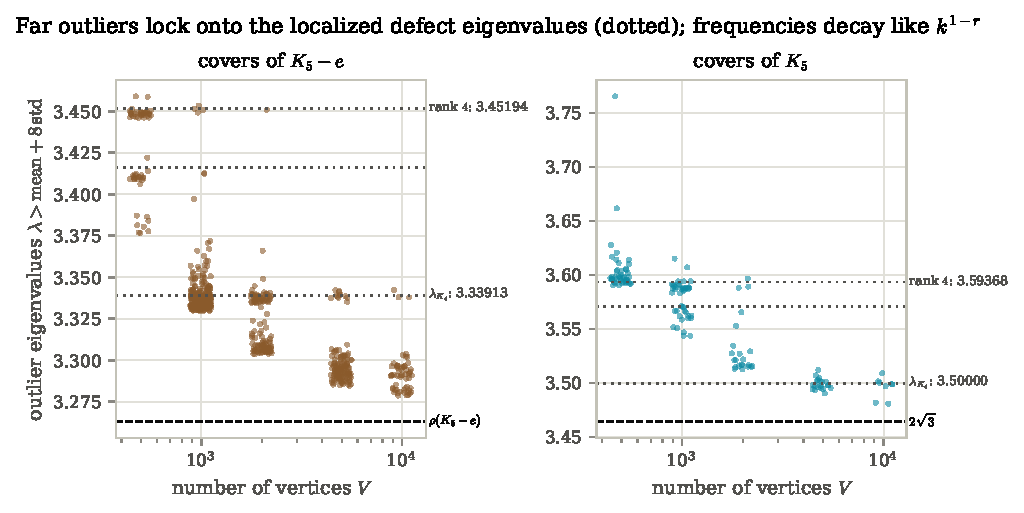
\includegraphics[width=0.95\columnwidth]{images/outlier_atoms_k5_families.pdf}
\par\end{centering}
\caption{\label{fig:atoms}Every sample more than eight standard deviations
above the mean, against $V$, for the $K_{5}-e$ (left) and $K_{5}$
(right) cover families, with the computed defect eigenvalues overlaid:
the outliers lock onto the $K_{4}$ atoms, $3.33913\dots$ for $K_{5}-e$
and exactly $7/2$ for $K_{5}$, and onto the cycle rank four values
(dotted), while the continuum of $K_{4}$ subdivisions drains toward
$\rho$ and the frequencies decay like $k^{1-r}$.}
\end{figure}

\begin{figure}[tbp]
\begin{centering}
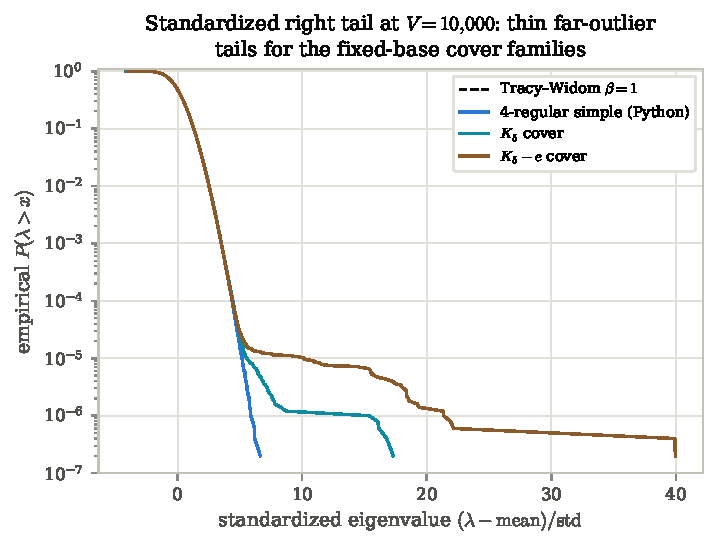
\includegraphics[width=0.7\columnwidth]{images/tail_survival_standardized_k5_families_V10000.pdf}
\par\end{centering}
\caption{\label{fig:tail_k5}Standardized right tail $P(\lambda>x)$ at $V=10{,}000$
for the simple $4$-regular, $K_{5}$ cover, and $K_{5}-e$ cover families.
The bulk of all three collapses onto the Tracy-Widom $\beta=1$ tail,
while the $K_{5}-e$ family carries a thin far outlier tail at frequency
near $10^{-5}$, reaching $42$ standard deviations, and the $K_{5}$
family a much thinner one.}
\end{figure}

\subsection{\label{subsec:k4e}The Boundary Case $K_{4}-e$}

The third fixed base, $K_{4}-e$, tests Conjecture \ref{conj:irregular_base}
at its boundary: the complete graph on four vertices minus an edge
has cycle rank exactly two, degrees $\left(2,3,3,2\right)$, and the
closed form
\[
\rho(K_{4}-e)=\sqrt{1+2\sqrt{7}}=2.5082867902\dots.
\]
Suppressing its two degree two vertices identifies $K_{4}-e$ with
the theta graph, two vertices joined by three parallel edges, and
so random covers of $K_{4}-e$ are subdivisions of random theta covers,
which are exactly the bipartite cubic multigraphs built from three
independent uniform permutations, the bipartite model of MNS and of
Novikoff's experiments \cite{Novikoff2002}. We sampled $10^{6}$
covers per size at the same seven sizes $V=4k$ between $100$ and
$10{,}000$.

The family fits the framework, and it converges more slowly than any
other. The mean approaches $\rho$ from below with the ratio $g_{V}$
rising through $0.7326$ at $V=10{,}000$ and the Ramanujan probability
through $0.79490$, both far from their conjectured limits $\left|\mu_{TW_{1}}\right|/\sigma_{TW_{1}}$
and $F_{1}(0)$. Two separate causes slow it down. The first is the
scale. The square root edge of $\mu_{K_{4}-e}$ is steep, $C_{B}=10.207$,
and narrow: $\pi\,\mu_{B}'(x)/\sqrt{\rho-x}$ is within $3\%$ of $C_{B}$
only within about $10^{-3}$ of the edge, against about $10^{-2}$
for $K_{5}-e$ (Figure \ref{fig:universal_cover}), and the fluctuation
scale $C_{B}^{-2/3}V^{-2/3}$ enters this window only at $V\approx3000$.
Accordingly the fitted amplitude descends slowly, through $0.2382$,
$0.2275$, and $0.2219$ at $V=2000$, $5000$, and $10{,}000$, and
extrapolates to $0.214$ to $0.216$ against the predicted $C_{B}^{-2/3}=0.212519$,
consistent with the prediction but with a larger uncertainty than
for $K_{5}-e$ (Figure \ref{fig:irregular_amplitude}). The second
cause is the far tail. The raw distributional statistics are contaminated
in a way the other covers only hint at: the excess kurtosis grows
to $12.7$, and the Kolmogorov-Smirnov distance of the standardized
sample to $\widetilde{TW}_{1}$, after falling to $3.8\times10^{-3}$
at $V=500$, grows again to $1.9\times10^{-2}$ at $V=10{,}000$ (Figure
\ref{fig:k4e}, left). Removing the tail, by discarding the $0.2\%$
of samples beyond six standard deviations, restores $\widetilde{TW}_{1}$
as the nearest law from $V=1000$ on, with distance $4.0\times10^{-3}$
at $V=10{,}000$ against $6.4\times10^{-3}$ and $9.9\times10^{-3}$
for $\widetilde{TW}_{2}$ and $\widetilde{TW}_{4}$, and the affine
quantile fit, which never sees the tail, gives $2.8\times10^{-3}$.

The tail itself differs from the $K_{5}-e$ tail exactly as the defect
picture predicts. No cycle rank one subgraph binds an eigenvalue above
$\rho$, and no connected $2$-cover of $K_{4}-e$ has a new eigenvalue
above $\rho$ either, as a direct check of all $32$ signings shows,
however the base now has cycle rank two, and so proper rank two subgraphs
exist, generalized thetas whose routes are longer than the base's
and which carry branches, occurring at the rate $k^{-1}$ of Proposition
\ref{prop:defect_counting}: the two shortest, $\theta(2,2,4)$ and
$\theta(1,2,5)$ in the notation of Table \ref{tab:defect_catalogue},
bind at
\[
2.5118521\dots\ \ \ \text{and}\ \ \ 2.5136918\dots,
\]
computed by the same branch recursion, one power of $k$ more frequent
than the leading $K_{5}-e$ defects. Above the rank two band, rank
three shapes reach $\approx2.530$ at rate $k^{-2}$. The data shows
precisely this structure (Figure \ref{fig:k4e}, right): the outliers
form a dense band draining toward $\rho$ rather than isolated atoms,
capped near $2.530$ at the largest sizes, with the count above the
rank two cap decaying with fitted exponent $1.96$ and the count at
the cap decaying visibly more slowly, still descending toward the
predicted $1$. In the notation of Conjecture \ref{conj:defect_completeness},
$r(\epsilon)=2$ for $\epsilon$ below $\approx0.006$ and $3$ up
to $\approx0.022$. The comparison across the three fixed bases is
the point: the denser the base, the higher the cycle rank at which
the defect hierarchy starts, and the further the atoms sit from $\rho$.
For $K_{4}-e$ the hierarchy starts at rank two, the band crowds the
bulk at accessible sizes, and the moments and even the raw Kolmogorov-Smirnov
distance feel it, which together with its narrow square root edge
is why this family, at the boundary of the conjecture, converges last.

\begin{figure}[tbp]
\begin{centering}
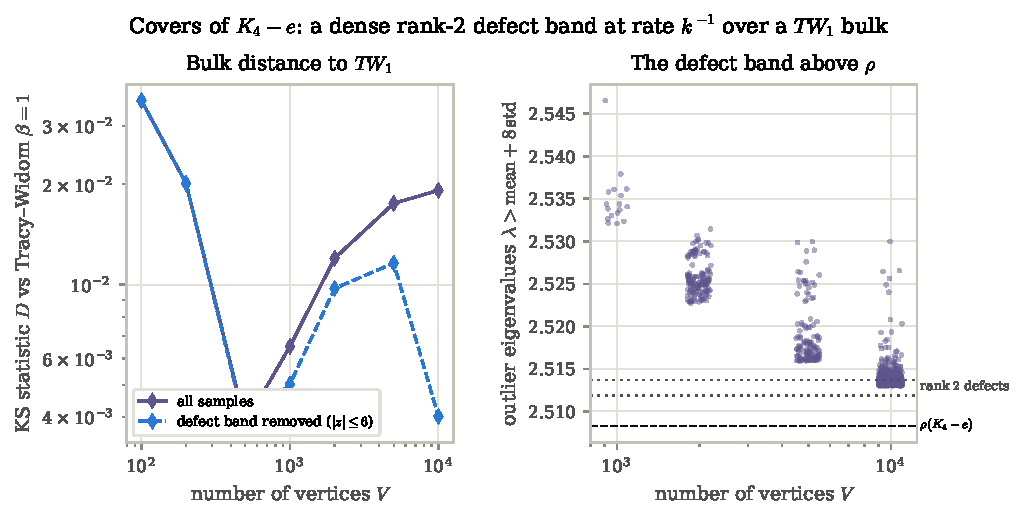
\includegraphics[width=0.95\columnwidth]{images/k4_minus_edge_bulk_and_defect_band.pdf}
\par\end{centering}
\caption{\label{fig:k4e}Covers of $K_{4}-e$. Left: Kolmogorov-Smirnov distance
of the standardized sample to $\widetilde{TW}_{1}$, for all samples
and with the defect band removed. Right: every sample more than eight
standard deviations above the mean against $V$, with $\rho(K_{4}-e)$
dashed and the two computed rank two defect eigenvalues dotted. The
band drains toward $\rho$ at rate $k^{-1}$, with rank three shapes
reaching $\approx2.530$ at rate $k^{-2}$.}
\end{figure}


\section{\label{sec:open_problems}Open Problems}

\subsection*{The Block Laws}

Conjecture \ref{conj:symmetry_classes} is open in every case, including
$\beta=1$: for covers of a $d$-regular base of size $n\geq2$ no
analog of Theorem \ref{thm:hmy} is known, and for irregular bases
even the correct formulation of edge rigidity around $\rho(B)$ is
open. The abelian case seems the natural first target, since the block
$A_{\chi}$ is an explicit random Hermitian matrix built from a random
regular graph and independent uniform phases, and the loop equation
approach, which characterizes the Airy$_{\beta}$ statistics for every
rational $\beta$ and has already given a simplified proof of Theorem
\ref{thm:hmy} \cite{BourgadeHuang2026}, seems well suited to it
(see also \cite{HuangYau2026}).
\begin{problem}
\label{prob:abelian_block}Prove that the largest eigenvalue of the
$\mathbb{Z}_{3}$-character block $A_{\chi}$ of a random $\mathbb{Z}_{3}$-cover
of a random simple $d$-regular graph has $TW_{2}$ fluctuations,
in the sense of Conjecture \ref{conj:symmetry_classes}.
\end{problem}

\subsection*{The Scale and the Location}

All of the scale constants in our data are predicted by the square
root edge of the limiting spectral measure, with the Gaussian ensembles
normalized alike, and the prediction is confirmed to within $0.15\%$
after extrapolation for $K_{5}$ and $K_{5}-e$. The location is a
different matter. The shift $a/n$ of (\ref{eq:finite_size_law})
has a family dependent constant, from $4.47$ for the simple $4$-regular
graphs to $-1.44$ for the multigraph and nearly $0$ for the covers
of $K_{5}$, and it controls the approach of every Ramanujan probability
to its limit, at rate $n^{-1/3}$.
\begin{problem}
\label{prob:location}Determine the location coefficient $a$. In
particular, is $a$ determined by the expected numbers of short cycles
of the model, as the $1/n$ corrections to the Kesten-McKay density
computed by Metz, Parisi, and Leuzzi \cite{MetzParisiLeuzzi2014}
suggest, and does the difference of about $6$ between the simple
and multigraph models come from the conditioning on the absence of
loops and double edges?
\end{problem}
I believe that the shift is a deterministic consequence of the short
cycles, since in the families of our data it changes when the cycle
statistics are changed and not otherwise, but I do not know how to
compute it.

\subsection*{Far Outliers}

The permutation multigraph model of subsection \ref{subsec:multigraph}
has the Tracy-Widom bulk of the simple model together with a thin
tail of defects of cycle rank two, and the fixed base families of
section \ref{sec:irregular} carry tails of the same character.
\begin{problem}
\label{prob:multigraph}Prove that the largest non-trivial eigenvalue
of the permutation multigraph model, rescaled as in Theorem \ref{thm:hmy},
converges to $TW_{1}$ in distribution. Is the point process of its
eigenvalues above $2\sqrt{3}+\epsilon$ asymptotically a Poisson process
on the three defect eigenvalues of subsection \ref{subsec:multigraph},
with total intensity of order $1/V$?
\end{problem}

\begin{problem}
\label{prob:outlier_rate}Prove the upper bound in Conjecture \ref{conj:defect_completeness}:
that nothing but the defects of subsection \ref{subsec:defects} inhabits
the polynomial tail. The lower bound is Proposition \ref{prop:defect_eigenvalue},
the regular Ramanujan case is the theorem of Friedman and Kohler \cite{FriedmanKohler2014,FriedmanKohler2019},
and the fitted exponents of subsections \ref{subsec:defects} and \ref{subsec:k4e}
match the conjectured rates on two irregular bases with different
leading ranks.
\end{problem}

\subsection*{Growing Covers}

Huang and Yau \cite{HuangYau2023} proved Tracy-Widom fluctuations
for regular graphs of growing degree. The analogous regime for covers,
base size fixed and cover group growing, is precisely the setting
of Conjecture \ref{conj:irregular_base}, however one may also grow
the base: for $\mathbb{Z}_{k}$ covers with $k$ growing with $n$,
the number of GUE blocks grows, and the largest new eigenvalue becomes
the maximum of a growing number of Tracy-Widom variables. The maximum
of independent Tracy-Widom variables lies in the Gumbel domain of
attraction \cite{ChetelatNarayananWells2018}, which suggests a transition
from Tracy-Widom to Gumbel fluctuations in the spirit of \cite{Johansson2007}.
For iterated $2$-covers of dense random regular graphs, Liu and Zou
\cite{LiuZou2025} prove exactly this maximum of independent Tracy-Widom
structure.
\begin{problem}
\label{prob:gumbel}For random $\mathbb{Z}_{k}$ covers of a random
$d$-regular graph on $n$ vertices, determine the joint regimes of
$(k,n)$ in which the largest new eigenvalue has Tracy-Widom, and
Gumbel, fluctuations.
\end{problem}

\specialsection*{Acknowledgements}

I would like to thank Lior Silberman, jointly with whom the conjectures
of this paper were formulated in 2018, for years of discussions about
this project. I would also like to thank Peter Sarnak for suggesting
the problem of the distribution of new eigenvalues of random covers,
and Stefan Glock for helpful correspondence regarding Sodin's work
and the scaling constants.

\bibliographystyle{plain}
\bibliography{references}

\end{document}
